\documentclass[twoside,11pt]{article}

% JMLR style. For submission, keep [preprint] off and fill \jmlrheading
% with placeholders; the editorial office sets volume/pages on acceptance.
\PassOptionsToPackage{hypertexnames=false}{hyperref}
\usepackage{xr-hyper}
\usepackage[abbrvbib]{jmlr2e}
% jmlr2e's proof environment takes no optional argument; allow one.
\renewenvironment{proof}[1][Proof]{\par\noindent{\bfseries #1\ }\ignorespaces}{\leavevmode\unskip\penalty9999\hbox{}\nobreak\hfill\quad\hbox{\BlackBox}\par\vspace{2mm}}

\usepackage{amsmath}
\usepackage{mathtools}
\usepackage{bm}
\usepackage{booktabs}
\usepackage{array}
\usepackage{microtype}
\usepackage{needspace}
\usepackage{xcolor}
\usepackage{algorithm}
\usepackage[noend]{algpseudocode}
\usepackage{enumitem}
\usepackage{placeins}
\usepackage{lastpage}
\usepackage[capitalise,nameinlink]{cleveref}
\hypersetup{pdftitle={Measuring Pairwise Diversity with Linearly Many Comparisons},
  pdfauthor={Shawn Ray},
  pdfkeywords={diversity, incomplete U-statistics, experimental design, multi-agent reinforcement learning, evaluation of generative models}}
\setlist{itemsep=2pt,topsep=4pt}
% Float spacing (vertical whitespace around figures and tables; JMLR 50-page rule)
\setlength{\textfloatsep}{12pt plus 2pt minus 4pt}
\setlength{\floatsep}{10pt plus 2pt minus 2pt}
\setlength{\intextsep}{10pt plus 2pt minus 2pt}
\setlength{\abovecaptionskip}{5pt}
\renewcommand{\topfraction}{0.9}
\renewcommand{\textfraction}{0.08}
\renewcommand{\floatpagefraction}{0.85}
\setcounter{topnumber}{3}
% Experimental details and additional results are in supplement.tex
% (labels prefixed S); build main, supplement, then main again.
\externaldocument{supplement}

% ---------- Notation ----------
\newcommand{\R}{\mathbb{R}}
\newcommand{\E}{\mathbb{E}}
\newcommand{\Prob}{\mathbb{P}}
\DeclareMathOperator{\Var}{Var}
\DeclareMathOperator{\rank}{rank}
\DeclarePairedDelimiter{\abs}{\lvert}{\rvert}
\DeclarePairedDelimiter{\norm}{\lVert}{\rVert}
% \SND denotes the population diversity mu(D) of any dissimilarity table;
% the MARL instance is written \mathrm{SND} explicitly.
\newcommand{\SND}{\mu}
\newcommand{\SNDG}{\widehat{\mu}_{G}}
\newcommand{\Pairs}{\mathcal{P}}
\newcommand{\sigmamain}{\sigma^2_{\mathrm{main}}}
\newcommand{\sigmaint}{\sigma^2_{\mathrm{int}}}
\newcommand{\sigmatot}{\sigma^2_{\mathrm{tot}}}
\newcommand{\SNDdes}{\mu_{\mathrm{des}}}
\newcommand{\muhat}{\widehat{\mu}}
\newcommand{\Dmat}{\mathbf{D}}
\newcommand{\Rmat}{\mathbf{R}}
\newcommand{\one}{\mathbf{1}}
\newcommand{\Sym}{\mathfrak{S}}

\jmlrheading{XX}{2026}{1-\pageref{LastPage}}{11/26}{--}{XX-XXXX}{Shawn Ray}
\ShortHeadings{Measuring Diversity with Linearly Many Comparisons}{Ray}
\firstpageno{1}

\raggedbottom
\brokenpenalty=10000
\emergencystretch=1.5em
\hyphenation{Cob-bold Theorem Theorems Proposition Propositions Corollary Corollaries Section Sections Appendix Appendices PyTorch NumPy Dieng Bettini November}
\begin{document}

\title{Measuring Pairwise Diversity\\ with Linearly Many Comparisons}

\author{\name Shawn Ray \email shawnray@cmu.edu \\
       \addr Carnegie Mellon University\\
       5000 Forbes Avenue\\
       Pittsburgh, PA 15213, USA}

\editor{}

\maketitle

\begin{abstract}%
Diversity is often measured as the average pairwise dissimilarity of $n$
agents, models, or generated outputs. Exact evaluation needs quadratically
many comparisons, and its single number hides how diversity is
organized. We use the classical decomposition, or anatomy, of
a pairwise table into a level, individual distinctiveness, and relational
structure such as roles. The error of any subset-of-pairs average is
exactly a distinctiveness term plus a relational term, and the first
vanishes for every population if and only if each individual is compared
equally often. With random labels, such balanced designs are unbiased, with
closed-form variance set by relational structure alone. For every metric,
$m$ such comparisons have relative root-mean-square error at most
$m^{-1/2}$, so ${O(n+\varepsilon^{-2})}$ comparisons fixed in advance give
relative error $\varepsilon$ with constant probability, an optimal rate
previously reached, to our knowledge, only adaptively; uniform pair sampling
can need about $n/2$ times more. On trained multi-agent teams, classifier
populations, and judge-scored language-model outputs, balanced designs need
up to seven times fewer comparisons than uniform pairs; with a
frontier-model judge, $128$ of $2{,}016$ calls estimate the diversity of
$64$ responses with $1$--$2\%$ root-mean-square error. The anatomy also
separates two multi-agent tasks by how their diversity develops.
\end{abstract}

\begin{keywords}
  diversity, incomplete U-statistics, experimental design,
  multi-agent reinforcement learning, evaluation of generative models
\end{keywords}

% ======================================================================
\section{Introduction}
\label{sec:intro}

Scoring every pair of $1{,}000$ language-model responses with a learned
judge takes at least $499{,}500$ judge calls, and it produces a single number, the
\emph{average pairwise dissimilarity} of the population,
\begin{equation}
  \mu(D) \;=\; \binom{n}{2}^{-1}\sum_{i<j} d_{ij},
  \label{eq:intro-mu}
\end{equation}
where $n$ is the population size and the table $D=(d_{ij})$ collects the
dissimilarities $d_{ij}\ge 0$ between individuals $i$ and $j$. The same statistic is a standard measure of diversity across
machine learning. It, or a close relative, scores the
diversity of generated text and molecules
\citep{zhu2018texygen,polykovskiy2020molecular,kirk2024understanding} and
the disagreement of ensemble members \citep{kuncheva2003measures}. In
multi-agent reinforcement learning (MARL), System Neural Diversity
\citep[SND;][]{bettini2025snd} is exactly \eqref{eq:intro-mu} with $d_{ij}$
the Wasserstein distance between two agents' action distributions, averaged
over a set of observations, and
Diversity Control (DiCo) holds it at a set point during training
\citep{bettini2024dico}. Up to a factor $(n-1)/n$, the average \eqref{eq:intro-mu} is also Rao's
quadratic entropy in ecology \citep{rao1982diversity} and nucleotide
diversity in population genetics \citep{nei1979mathematical}. Diversity
also matters for learning systems: teams of behaviorally diverse agents
specialize, explore better, and are more resilient to noise and
disturbances \citep{bettini2023hetgppo,bettini2024dico,bettini2025snd}, diverse deep ensembles are
better calibrated \citep{lakshminarayanan2017simple}, and diverse
populations of policies explore more effectively
\citep{lehman2011abandoning,parker-holder2020effective}.

The average pairwise dissimilarity has two limitations that grow with the
population. The first is cost. It needs $\binom{n}{2}$ comparisons, and a
single comparison is often expensive: a Wasserstein distance averaged over
thousands of observations, a divergence between two networks' predictions
on a test set, a transport or edit distance, a rollout, or a call to a
learned judge. When diversity is computed at every
training iteration or fed back into a controller, this quadratic tax
can become the bottleneck. The second limitation is opacity. The same average
can be produced by a population in which everyone is moderately different, by
one with two internally homogeneous roles, and by one with a single
outlier. These are different phenomena with different consequences, and a
scalar cannot tell them apart.

We show that a classical structural fact addresses both limitations.
\Cref{thm:anatomy} \citep{griffing1956concept,james1978representation}
states that every dissimilarity table decomposes uniquely as
\begin{equation}
  d_{ij} \;=\; \underbrace{\mu}_{\text{level}}
  \;+\; \underbrace{a_i + a_j}_{\text{distinctiveness}}
  \;+\; \underbrace{r_{ij}\mathrlap{,}}_{\text{relations}}
  \qquad \textstyle\sum_i a_i = 0,\quad \sum_{j\ne i} r_{ij}=0 \ \ \forall i,
  \label{eq:intro-anatomy}
\end{equation}
into three mutually orthogonal parts. The level $\mu$ is the average
itself. The distinctiveness $a_i$ measures how much farther individual $i$
is from everyone else than a typical individual is. The relational part
$r_{ij}$ is what remains once level and distinctiveness are accounted for:
which particular pairs are unexpectedly similar or different, as happens
with roles and clusters. We call this decomposition the \emph{anatomy} of
the table. It is canonical: the three parts are the only components that
relabeling the individuals cannot mix, so whenever the compared pairs are
chosen without regard to the labels, the variance of their average depends
on the table only through the mean squares of the distinctiveness and
relational parts (\Cref{sec:anatomy}). \Cref{fig:teaser}(a) shows the
anatomy of a small team.

\begin{figure}[t]
  \centering
  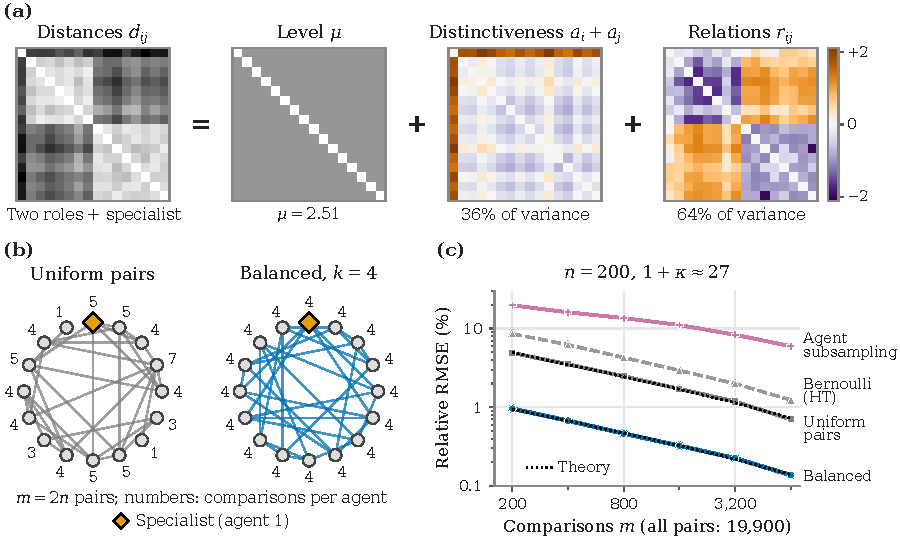
\includegraphics[width=\textwidth]{figures/fig1_teaser.pdf}
  \caption{\textbf{The anatomy of pairwise diversity sets the cost of
  measuring it.} (a) A synthetic team of $n=16$ agents with two behavioral
  roles and one specialist (agent~1). Its distance table splits uniquely into
  a level (the diversity $\mu$), the distinctiveness table $a_i+a_j$, and
  relational structure $r_{ij}$ (\Cref{thm:anatomy}). Gray runs from $0$
  (white) to the largest distance; the last two panels share one symmetric
  color scale (orange positive, purple negative), and the percentages are
  their shares of the pairwise variance. (b) Two designs with the same budget
  of $m=2n$ pairs. Uniform pair sampling compares one agent seven times and
  two agents only once; a balanced design compares every agent exactly $k=4$
  times. (c) Relative root-mean-square error (RMSE) of the estimated
  diversity of a synthetic $200$-member population with heterogeneous
  distinctiveness ($1+\kappa\approx27$, where $\kappa$ is the ratio of
  distinctiveness to relational energy), over $2{,}000$ design draws, for
  agent subsampling (all pairs within a random subset), Bernoulli sampling
  with the Horvitz--Thompson (HT) estimator, uniform pairs, and the balanced
  design (permuted circulant). Balanced designs cancel the distinctiveness
  term exactly (\Cref{prop:error-identity}), so uniform pairs have about $27$
  times more variance at every budget (\Cref{cor:efficiency}); dotted lines
  are the closed-form predictions of \Cref{thm:balanced,cor:efficiency}.}
  \label{fig:teaser}
\end{figure}

The anatomy turns sparse estimation of $\mu$ into a question with an exact
answer. Suppose we compare only the pairs in a graph $G$ and average them.
\Cref{prop:error-identity} shows that the error equals a
\emph{distinctiveness leakage}, which is proportional to the covariance
between how often
an individual is compared and how distinctive it is, plus a
\emph{relational leakage}, which is the average residual on the compared
pairs. The first term vanishes for every population if and only if every
individual is compared equally often (\Cref{prop:regular-necessary}). This
observation leads to the designs we study, \emph{randomized balanced
designs}:\footnote{Here \emph{balanced} means that every individual is
compared equally often (an equireplicate design). In the sense of balanced
incomplete block designs, the only balanced design with blocks of size two
is the complete graph.} draw
a random relabeling of the population, then compare each individual with
its $k$ neighbors in a fixed $k$\nobreakdash-regular pattern
(\Cref{fig:teaser}(b)), such as a ring lattice (the \emph{permuted circulant} of
\Cref{alg:balanced}) or $k$ rounds of a round-robin schedule (the
\emph{round-robin design}). These designs have four properties.
\begin{itemize}
  \item \textbf{Exact and closed-form.} The estimate is exactly unbiased,
  and with $m=nk/2$ comparisons its variance is
  $\sigmaint\,(n-1-k)/\bigl(m(n-3)\bigr)\approx2\sigmaint/(nk)$, which
  depends on the population only through the relational energy $\sigmaint$,
  the mean squared relational residual (\Cref{thm:balanced}).
  \item \textbf{Efficiency set by the anatomy.} At equal cost, uniform pair
  sampling has about $1+\kappa$ times the variance, where $\kappa$ is the
  ratio of distinctiveness energy to relational energy; uniform sampling can
  win only when $\kappa=O(1/n)$, and then by a factor $1+O(1/n)$
  (\Cref{cor:efficiency}).
  \item \textbf{Universal and optimal.} The triangle inequality bounds the
  relational energy by ${(n-2)\mu^2/n}$, a bound attained for every even $n$.
  Hence, for every metric, a balanced design with $m$ comparisons has relative
  root-mean-square error at most $m^{-1/2}$, and
  ${O(n+\varepsilon^{-2})}$ comparisons give relative error $\varepsilon$
  with constant probability and with no further assumption on the population (\Cref{thm:metric}). This rate is
  optimal for constant failure probability, and uniform pair sampling can
  require about $n/2$ times as many comparisons (\Cref{prop:lower}).
  \item \textbf{Informative.} The same comparisons give unbiased estimates
  of every individual's distinctiveness (\Cref{prop:sparse-anatomy}) and,
  for the round-robin design, an exactly unbiased variance estimate
  (\Cref{prop:rr-variance}).
\end{itemize}
For a fixed comparison graph, \Cref{thm:fixed-spectral} bounds the error
of any $k$\nobreakdash-regular graph by its spectrum and the relational part
alone, and \Cref{prop:error-identity} shows exactly how local interaction
graphs, such as nearest-neighbor or communication graphs, under-report
diversity: through negative residuals on the compared pairs and by
over-representing typical individuals.
Finally, \Cref{prop:dico} shows that, at each control step, a DiCo-type
controller inherits the relative error of the estimate to first order.

We test these results on synthetic populations that isolate each
anatomical component, on multi-agent teams trained with independent
proximal policy optimization \citep[PPO;][]{schulman2017proximal,dewitt2020independent}
in the Vectorized Multi\nobreakdash-Agent Simulator \citep[VMAS;][]{bettini2022vmas},
on populations of $128$ and $1{,}024$ trained classifiers, on
language-model outputs scored by neural judges, and in closed-loop
diversity control (\Cref{sec:experiments}). Simulations confirm the closed
forms to within Monte Carlo error (\Cref{fig:teaser}(c), \Cref{fig:laws},
and \Cref{sec:exp-judge}), and the anatomy predicts the gains on real
populations: at equal cost, the balanced design has up to $7.2$ times less
variance than uniform pair sampling on trained teams (median $2.4$; slightly
less, within the factor of \Cref{cor:efficiency}, when diversity is almost
purely relational),
$1.5$--$1.6$ times less on classifier populations, $1.6$--$3.8$ times less on
single-prompt populations of generated text, and up to two orders of
magnitude less when a few individuals are outliers; the adaptive optimal-rate scheme of
\citet{chechik2015average} is $1.4$--$10$ times less accurate than the
balanced design at equal cost (\Cref{tab:e2}). With
Claude Opus 5.5 as the judge, $128$ calls (about $\$0.25$) estimate the
diversity of $64$ generated responses with a relative root-mean-square error
of $1.05\%$, whereas all $2{,}016$ pairs cost $\$3.93$. One design per temperature, with
its own error bar, traced a Claude-judged diversity curve over six
temperatures with $1{,}000$ responses each for $\$28.80$ instead of about
$\$6{,}000$ (\Cref{fig:judge}(c)). Inside DiCo, $50$ agents trained with a balanced
design that uses a tenth of the comparisons per call show no detectable loss
of tracking or reward (\Cref{sec:exp-control}).

The anatomy is informative in its own right: SND reports only that diversity
grows in two VMAS tasks, but the anatomy shows distinctiveness dominating in
Navigation and giving way to relational structure in Dispersion, with
independent or centralized critics (\Cref{sec:exp-anatomy}); in a classifier population the relational part
recovers the four training recipes exactly, and the most distinctive
generated responses include refusals, a switch of language, and an
off-topic story (\Cref{sec:exp-zoo,sec:exp-judge}).

\paragraph{Contributions.}
Our contributions are (i) the sharp bound ${\sigmaint\le(n-2)\mu^2/n}$,
which is a classical consequence of the triangle inequality written in
anatomy coordinates and shows that a non-adaptive, equally weighted design
with $m$ comparisons has relative root-mean-square error at most $m^{-1/2}$
for every pseudometric and reaches the optimal rate
(\Cref{thm:metric,prop:lower});
(ii) for a fixed population, the exact error of every design and the anatomy-based variance of
every relabeled design, which give the efficiency of balanced designs
over uniform pairs and the threshold below which irregular designs do
better (\Cref{prop:error-identity,thm:balanced,cor:efficiency,thm:general-design});
(iii) the anatomy as a diagnostic of how diversity is organized, a
spectral guarantee for fixed designs that holds for every table, and a per-step tracking bound for
diversity control (\Cref{sec:anatomy,thm:fixed-spectral,prop:dico}); and
(iv) experiments on synthetic populations, multi-agent teams, model
populations, and language-model outputs scored by neural judges, which
verify the closed forms, measure the gains over uniform and adaptive
sampling on real populations, and show what the anatomy reveals
(\Cref{sec:experiments}), and a NumPy implementation
(\Cref{sec:discussion}).

\paragraph{What is classical.}
Several ingredients are classical. The decomposition
\eqref{eq:intro-anatomy} is the two-way analysis of variance of a
symmetric table \citep{griffing1956concept} and the finite-population
Hoeffding decomposition of a degree-two U-statistic
\citep{nandi1963properties,bloznelis2001orthogonal}, and its relational
part is the U-centered matrix of distance covariance
\citep{szekely2014partial}. The inequality behind our metric bound appears,
for Euclidean data, in the proof that the distance standard deviation is at
most Gini's mean difference \citep{edelmann2020distance}. The variance of a
uniformly relabeled design is a
permutation moment of a quadratic-assignment statistic
\citep{mantel1967detection}. The permuted circulant is the circulant partial
diallel cross of \citet{kempthorne1961partial}; like the round-robin
pattern, it is an equireplicate design for incomplete U-statistics
\citep{lee1982incomplete,miglioli2025incomplete}, and such designs minimize
the variance for i.i.d.\ data \citep{blom1976some,lee1982incomplete}. For
$k=1$ the design is a uniformly random perfect matching, whose total
distance \citet{chang2017metric} analyzed in metric spaces. The sparse distinctiveness
estimates rest on the textbook estimator of simple random sampling
\citep{cochran1977sampling}. The
lower-bound constructions follow \citet{barhum2007approximating}, who also gave
deterministic expander guarantees for $\ell_1$-embeddable tables, and the rate
$O(n+\varepsilon^{-2})$ was first reached, adaptively and with unequal weights,
by \citet{chechik2015average}; see \Cref{sec:related}. In survey-sampling
terms, the error identity (\Cref{prop:error-identity}) is the regression
decomposition with the individual-incidence vectors as auxiliary variables
\citep{sarndal1992model}, regular designs are balanced samples on those
vectors \citep{deville2004efficient}, \Cref{thm:balanced}(iii) makes the
balanced-sampling variance approximation of \citet{deville2005variance}
exact for relabeled designs, and the round-robin variance estimate is the
random-group estimator \citep{wolter2007introduction}. What is new is
therefore not the decomposition or its moments but their consequences for a
fixed population, listed above.

\paragraph{Scope.}
Our results apply to any symmetric, non-negative dissimilarity; only the
universal budget uses the triangle inequality. Squared Hilbert-space
distances (squared Euclidean, cosine, or squared Hellinger distance, learned
perceptual image patch similarity [LPIPS; \citealp{zhang2018unreasonable}],
or classifier disagreement) admit an exact linear-time formula
(\Cref{prop:separable} in the Supplementary Material). Our designs target the
many dissimilarities without one, such as the Wasserstein distance behind
SND, transport and edit distances, and rollout- or judge-based comparisons,
and need only black-box access to $d$.

% ======================================================================
\section{Setting: Pairwise Diversity and Comparison Designs}
\label{sec:setting}

\paragraph{Populations and dissimilarities.}
A population consists of $n\ge 4$ individuals, indexed by $[n]=\{1,\dots,n\}$.
Let $\Pairs=\{\{i,j\}:1\le i<j\le n\}$ be the set of unordered pairs and
$N=\abs{\Pairs}=\binom{n}{2}$. A \emph{dissimilarity table} is a symmetric
matrix $D=(d_{ij})\in\R^{n\times n}$ with $d_{ii}=0$ and $d_{ij}\ge 0$. It
is a \emph{pseudometric table} if, in addition, $d_{ij}\le d_{il}+d_{lj}$
for all $i,j,l$. The \emph{pairwise diversity} of the population is
\begin{equation}
  \SND(D) \;=\; \frac{1}{N}\sum_{i<j} d_{ij}.
  \label{eq:mu}
\end{equation}
We write $\SND$ for $\SND(D)$ when the table is clear, and $S_i=\sum_{j\ne
i}d_{ij}$ for the $i$-th row sum; $\one$ denotes the all-ones vector and $\R^{\Pairs}$ the space of real tables indexed by unordered pairs. Everything in this paper is conditional
on the population: $D$ is a fixed table, and all randomness comes from
which pairs we choose to compare. This is the right target when the
population is the object of interest, as for a team of agents, an ensemble,
or a set of checkpoints. \Cref{sec:discussion} discusses the case where the
individuals are themselves a sample from a larger distribution.

\needspace{5\baselineskip}
\paragraph{Three instances.} The theory applies to three kinds of population.
\begin{itemize}
  \item \emph{Behavioral diversity in MARL.} Agents $i\in[n]$ act through
  stochastic policies ${\pi_i(\cdot\mid o)}$ over a shared observation and
  action space. Following \citet{bettini2025snd}, the behavioral distance
  is
  \begin{equation}
    d_{ij} \;=\; \frac{1}{\abs{\mathcal{B}}}\sum_{o\in\mathcal{B}}
    W_2\bigl(\pi_i(\cdot\mid o),\,\pi_j(\cdot\mid o)\bigr),
    \label{eq:snd-distance}
  \end{equation}
  where $\mathcal{B}$ is a set of observations collected from rollouts and
  $W_2$ is the 2-Wasserstein distance, which has a closed form for Gaussian
  policies. With this distance, \eqref{eq:mu} is System Neural Diversity,
  $\mathrm{SND}=\SND(D)$. Sharing the observation and action spaces is an
  assumption inherited from SND: it is what makes any two policies
  comparable at the same observation. Evaluating all $n$ policies on
  $\mathcal{B}$ costs $O(n\abs{\mathcal{B}})$ forward passes, paid once by
  any design that touches every agent; each $d_{ij}$ then costs
  $O(\abs{\mathcal{B}})$ distance computations, which is what a sparse
  design saves. The distance $d$ is a pseudometric because $W_2$ is a metric. With
  total variation in place of $W_2$, as for categorical policies, $\SND$
  would be computable exactly in $O(n\log n)$ time per observation and
  action by sorting (\Cref{prop:separable}); Gaussian $W_2$ admits no such
  identity.
  \item \emph{Model populations.} Individuals are trained predictors, such
  as ensemble members, checkpoints, or the models produced by a hyperparameter sweep.
  Here $d_{ij}$ averages the Jensen--Shannon distance between their predictive
  distributions over an evaluation set. This is also a pseudometric.
  \item \emph{Any population with an expensive comparison.} Examples include
  embeddings compared by Euclidean distance, sequences compared by edit
  distance, point clouds compared by optimal transport, and generated texts
  compared by a learned judge that reads both texts at once.
\end{itemize}

\paragraph{Comparison designs.}
A \emph{comparison design} is a weighted graph $G=([n],E,w)$ with
$E\subseteq\Pairs$, weights $w_e\ge 0$, and total weight $W=\sum_{e\in
E}w_e>0$. It evaluates only the pairs in $E$ and reports
\begin{equation}
  \SNDG \;=\; \frac{1}{W}\sum_{e\in E} w_e\, d_e .
  \label{eq:design-estimator}
\end{equation}
The cost is $\abs{E}$ comparisons instead of $N$. We write
$\delta_i=\sum_{j:\{i,j\}\in E} w_{ij}$, with $w_{ij}=w_{\{i,j\}}$, for the weighted degree of $i$ and
$\bar\delta=2W/n$ for its average. For an unweighted design, $\delta_i$ is the
number of comparisons involving $i$ and ${W=m=\abs{E}}$. Designs can be
random or fixed. The complete graph recovers $\SND$ exactly. Bernoulli
sampling, which keeps each pair independently with probability $p$, and
uniform sampling of $m$ distinct pairs are the standard random designs.
Nearest-neighbor, communication, and spatial-proximity graphs are common
fixed designs. In MARL, \eqref{eq:design-estimator} with the distance
\eqref{eq:snd-distance} was introduced as \mbox{Graph-SND} \citep{ray2026graphsnd};
our results say which graphs to use and what each of them measures.

% ======================================================================
\section{The Anatomy of Pairwise Diversity}
\label{sec:anatomy}

The average \eqref{eq:mu} compresses $N$ numbers into one. To see what it
hides, and what a sparse estimate of it can miss, we split the table
into the parts that relabeling the individuals cannot mix.

\begin{definition}[Anatomy of a dissimilarity table]
\label[definition]{def:anatomy}
The \emph{distinctiveness} of individual $i$ and the \emph{relational
residual} of the pair $\{i,j\}$ are
\begin{equation}
\label{eq:anatomy-def}
a_i \;=\; \frac{S_i-(n-1)\mu}{n-2},
\qquad
r_{ij} \;=\; d_{ij}-\mu-a_i-a_j \quad (i\neq j),
\end{equation}
with $r_{ii}:=0$ and $R=(r_{ij})$. The total, distinctiveness (main-effect),
and relational (interaction) energies are
\[
\sigmatot=\frac{1}{N}\sum_{i<j}(d_{ij}-\mu)^2,\qquad
\sigmamain=\frac{1}{N}\sum_{i<j}(a_i+a_j)^2,\qquad
\sigmaint=\frac{1}{N}\sum_{i<j}r_{ij}^2.
\]
We write
$\kappa=\sigmamain/\sigmaint\in[0,\infty]$ for their ratio, with $\kappa:=0$
if $\sigmamain=0$ and $\kappa:=\infty$ if $\sigmamain>0=\sigmaint$.
\end{definition}

Since $S_i/(n-1)$ is the average dissimilarity between $i$ and the others,
$a_i$ is the excess of that average over $\mu$, rescaled by $(n-1)/(n-2)$. A positive $a_i$ marks an individual
that is far from everyone, such as a specialist or an outlier. A negative
$a_i$ marks a central, typical individual. The residual $r_{ij}$ is
positive for pairs that are more different than their distinctiveness
predicts and negative for pairs that are more alike, as happens within a
role. Since $r_{ij}=d_{ij}-(S_i+S_j)/(n-2)+n\mu/(n-2)$, the residual table
$R$ is exactly the \emph{U-centered} matrix of $D$ used for unbiased
distance covariance \citep{szekely2014partial}, and
$\sigmaint=\frac{n-3}{n-1}\,\Omega_n$, where
$\Omega_n=\frac{1}{n(n-3)}\sum_{i\neq j}r_{ij}^2$ is their unbiased
estimator of the squared distance variance when $D$ is a table of distances
between sample points.

The decomposition itself is classical (\Cref{sec:related}); we state it in
the form used throughout.

\begin{theorem}[Anatomy of diversity; \citealp{griffing1956concept,james1978representation}]
\label{thm:anatomy}
Every dissimilarity table $D$ satisfies the following.
\begin{enumerate}
\item[(i)] \emph{Existence and uniqueness.} $d_{ij}=\mu+a_i+a_j+r_{ij}$
for all $i\ne j$, with $\sum_i a_i=0$ and $R\one=0$. Conversely, if
$d_{ij}=\mu'+a'_i+a'_j+r'_{ij}$ for all $i\neq j$, with $\sum_i a'_i=0$,
$r'_{ii}=0$ for all $i$, and $R'\one=0$, then $(\mu',a',R')=(\mu,a,R)$.
\item[(ii)] \emph{Energy identity.} The level, distinctiveness, and
relational components are mutually orthogonal in $\R^{\Pairs}$. Hence
$\sigmatot=\sigmamain+\sigmaint$, and
$\sigmamain=\frac{n-2}{N}\sum_{i}a_i^2$.
\item[(iii)] \emph{Canonicity.} Under relabeling of the individuals by
the symmetric group $\Sym_n$, the space $\R^{\Pairs}$ splits into exactly three
irreducible invariant subspaces, of dimensions $1$, $n-1$, and $n(n-3)/2$.
They are the constants, the main-effect tables
$\{(a_i+a_j)_{i<j}:\sum_i a_i=0\}$, and the residual tables
$\{R:R\one=0\}$. The decomposition is multiplicity-free, so it is the only
decomposition of $\R^{\Pairs}$ into irreducible invariant subspaces.
\end{enumerate}
\end{theorem}

Parts (i) and (ii) are a two-way analysis of variance for a symmetric table
with an empty diagonal. They match the Hoeffding decomposition of a
U-statistic under sampling without replacement from a finite population \citep{nandi1963properties,bloznelis2001orthogonal}
and the symmetric social relations model of psychology
\citep{kenny1984social}. Part (iii) explains why this decomposition, and no
other, governs the error of every relabeling-invariant design: the space of
pairwise tables is the permutation module $M^{(n-2,2)}$ of $\Sym_n$, which
splits into the Specht modules $S^{(n)}\oplus S^{(n-1,1)}\oplus S^{(n-2,2)}$
\citep{james1978representation,diaconis1988group}, and by Schur's lemma any
linear operator that commutes with relabeling, such as the second-moment
operator of a uniformly relabeled design, acts as a scalar on each part. The
variance of every such design is therefore a combination of $\sigmamain$
and $\sigmaint$ with coefficients set by the design
(\Cref{thm:general-design,rem:schur} in \Cref{app:general-design}). In the
language of designed experiments, these are the strata of the triangular
association scheme on pairs \citep{bose1952classification}, and the
dependence of a randomized design's variance on stratum energies is the
randomization theory of \citet{bailey1991strata,bailey2004association}.
Proofs are in \Cref{app:proofs}, and \Cref{tab:notation} in the
Supplementary Material summarizes the notation.

\paragraph{Diagnostics.}
The anatomy turns one number into a profile: the \emph{level} $\mu$; the
\emph{distinctiveness share} $\sigmamain/\sigmatot$ and profile
$(a_i)_{i\in[n]}$, which say whether diversity is carried by a few
individuals and by which ones; the \emph{relational share}
$\sigmaint/\sigmatot$ and the spectrum of $R$, which reveal roles or
clusters; and the scale-free ratios $\sigma_{\mathrm{main}}/\mu$ and
$\sigma_{\mathrm{int}}/\mu$, which, as we show next, set the cost of
measuring $\mu$. Three populations can share the same $\mu$ while having very different anatomies:
one with ${\sigmamain\approx\sigmaint\approx 0}$ (everyone equally
different), one with $\sigmamain/\sigmatot\approx 1$ (a few outliers), and
one with $\sigmaint/\sigmatot\approx 1$ (roles). \Cref{fig:teaser}(a) shows
a team that has all three components. With $K$ well-separated roles,
${R\approx F-\operatorname{Diag}(F)}$ (with equality when $d_{ij}$ depends only on
the roles of $i$ and $j$), where the role-level table $F$ (constant
on blocks of individuals that share a role) has rank at most $K$, and
effectively $K-1$ because the constraint $R\one=0$ nearly centers it.
Because of its zero diagonal, $R$ generically has rank $n-1$, but its
$K-1$ leading eigenvectors indicate role membership, as in classical
scaling \citep{torgerson1952multidimensional,gower1966some}.

% ======================================================================
\section{Which Pairs Should We Compare?}
\label{sec:designs}

We first derive the exact error of any comparison design, and then use it
to construct randomized balanced designs (\Cref{sec:balanced}), give a
budget that holds for every metric (\Cref{sec:metric}), analyze fixed
designs (\Cref{sec:fixed}), estimate each individual's distinctiveness from the
same comparisons (\Cref{sec:sparse-anatomy}), and show how estimation error
propagates into closed-loop diversity control (\Cref{sec:control}).

\subsection{An exact error identity}

Substituting the anatomy into the design estimator
\eqref{eq:design-estimator} gives its error in closed form.

\begin{proposition}[Exact error identity]
\label[proposition]{prop:error-identity}
For every dissimilarity table $D$ and design $G$,
\begin{equation}
\label{eq:error-identity}
\SNDG-\SND
\;=\;
\underbrace{\frac{1}{W}\sum_{i=1}^n(\delta_i-\bar\delta)\,a_i}_{\textup{distinctiveness leakage}}
\;+\;
\underbrace{\frac{1}{W}\sum_{e\in E}w_e\,r_e\mathrlap{.}}_{\mathclap{\textup{relational leakage}}}
\end{equation}
\end{proposition}

The level cancels because $\SNDG$ is a weighted average. The distinctiveness
leakage is proportional to the covariance between how often an individual is compared and how
distinctive it is. The relational leakage is the weighted average residual
over the compared pairs. The identity is exact, holds for every design,
random or fixed, and needs no assumption on $D$. It shows at once what each
common design gets wrong.
\begin{itemize}
  \item A \emph{nearest-neighbor or communication graph} compares
  individuals that are close in some space. If proximity predicts
  behavioral similarity, the compared pairs have negative residuals, and
  the relational leakage is negative: the design systematically
  under-reports diversity. Individuals with many neighbors also dominate the
  average, so the design leaks distinctiveness as well. Such a design is
  better read as a measure of \emph{local} diversity than as an estimate of
  $\mu$ (\Cref{sec:fixed}).
  \item \emph{Uniform or Bernoulli pair sampling} is unbiased, but its
  degrees fluctuate. Each individual's random degree multiplies its
  distinctiveness, which adds variance proportional to $\sigmamain$.
  \item \emph{Agent subsampling}, which compares all pairs within a random
  subset of $s$ individuals, gives degree $s-1$ to the chosen individuals
  and $0$ to the rest. Its distinctiveness leakage is large, and its
  variance decays only like $m^{-1/2}$ in the number of comparisons.
\end{itemize}
The distinctiveness leakage, the first term of \eqref{eq:error-identity},
can be removed completely.

\begin{proposition}[Balance is necessary and sufficient]
\label[proposition]{prop:regular-necessary}
Fix a design $G$ and $\alpha>0$, and let $\mathcal{D}_\alpha$ be the set
of pseudometric tables whose anatomy has $R=0$ and
$\norm{a}_2\le\alpha$. Then
\[
\sup_{D\in\mathcal{D}_\alpha}\abs{\SNDG-\SND}
\;=\;\frac{\alpha\,\norm{\delta-\bar\delta\one}_2}{W}.
\]
Hence the error of $G$ is unaffected by distinctiveness, for every table,
if and only if $G$ is \emph{balanced}, that is, weighted-regular
($\delta_i\equiv\bar\delta$). For
unweighted designs this holds if and only if $G$ is regular, that is, if
every individual is compared equally often.
\end{proposition}

\subsection{Randomized balanced designs}
\label{sec:balanced}

A regular design removes distinctiveness, but a fixed regular graph can
still align with relational structure, for instance by comparing only
within roles. Randomizing the labels removes that risk.

\begin{algorithm}[t]
\caption{Balanced pairwise diversity (one design; repeat $L$ times for
intervals or high-probability guarantees)}
\label{alg:balanced}
\begin{algorithmic}[1]
\Require population $[n]$; dissimilarity oracle $d(\cdot,\cdot)$; degree $1\le k\le n-1$ with $nk$ even
\State Draw a uniformly random bijection $\sigma:\mathbb{Z}_n\to[n]$
\State $E\gets\bigl\{\{\sigma(t),\sigma(t+s)\} : t\in\mathbb{Z}_n,\ 1\le s\le \lfloor k/2\rfloor\bigr\}$
\Comment{permuted circulant}
\State \algorithmicif\ $k$ is odd \algorithmicthen\ $E\gets E\cup\bigl\{\{\sigma(t),\sigma(t+n/2)\} : 0\le t<n/2\bigr\}$ \Comment{$n$ is even here}
\State Evaluate $d_e$ for all $m=nk/2$ pairs $e\in E$ \Comment{the only expensive step; parallel}
\State $T\gets \frac{1}{m}\sum_{e\in E}d_e$ \Comment{diversity estimate}
\State $\widehat m_i\gets\frac1k\sum_{j:\{i,j\}\in E}d_{ij}$ and
$\widehat a_i\gets\frac{n-1}{n-2}(\widehat m_i-T)$ for all $i$
\Comment{distinctiveness estimates}
\State \Return $T$, $(\widehat a_i)_{i\in[n]}$, and the residuals
$\widehat r_{ij}=d_{ij}-T-\widehat a_i-\widehat a_j$ for $\{i,j\}\in E$
\end{algorithmic}
\end{algorithm}

\Cref{alg:balanced} is the simplest instance. It lays the relabeled
individuals on a circle and compares each with its $\lfloor k/2\rfloor$ nearest positions
on either side; odd $k$ (with $n$ even) adds the $n/2$ diametral pairs. It
belongs to the circulant partial diallel crosses of
\citet{kempthorne1961partial}, here applied to diversity measurement; all
relabeled circulant designs of the same degree have the same variance
(\Cref{thm:balanced}). A second instance, used for error bars
in \Cref{sec:exp-ci}, is the \emph{round-robin design}\footnote{In the social
relations model \citep{kenny1984social}, a round-robin design observes every
pair; here it means $k$ rounds of a round-robin tournament schedule.}: after a uniform
relabeling (for even $n$), the circle-method schedule partitions all $N$ pairs into $n-1$
rounds of $n/2$ disjoint pairs, and the design keeps $k$ rounds chosen
uniformly at random. The following theorem covers every such construction.

\begin{theorem}[Randomized balanced designs]
\label{thm:balanced}
Let $H$ be any simple $k$-regular graph on $[n]$ ($1\le k\le n-1$, $nk$
even), and let $\sigma$ be a uniformly random permutation of $[n]$. Set
$G=\sigma(H)$, $m=nk/2$, and $T=m^{-1}\sum_{e\in E(G)}d_e$. Then:
\begin{enumerate}
\item[(i)] $T-\SND=m^{-1}\sum_{e\in E(G)}r_e$ for every realization of $\sigma$;
\item[(ii)] $\E[T]=\SND$;
\item[(iii)] $\displaystyle \Var(T)=\frac{\sigmaint}{m}\cdot\frac{n-1-k}{n-3}$.
\end{enumerate}
The mean and the variance of the error depend on $H$ only through $(n,k)$.
In particular, $\Var(T)$ does not depend on the expansion of $H$, and
$\Var(T)=0$ when $k=n-1$. Higher moments of the error can depend on $H$.
All statements also hold when $H$ is random and independent of $\sigma$, as
for the round-robin design, since they hold conditionally on $H$.
\end{theorem}

In practice, the variance is exact and a single round-robin design
estimates it without bias (\Cref{prop:rr-variance}; \Cref{sec:exp-ci});
populations whose diversity is mostly level and distinctiveness are
measured almost exactly; and once the labels are randomized, regularity,
not expansion, determines the variance, so the simplest pattern is as
accurate in mean square as a Ramanujan expander.

\begin{corollary}[Efficiency over uniform pair sampling]
\label[corollary]{cor:efficiency}
Let $T_U$ be the mean of $d$ over $m$ pairs drawn uniformly without
replacement from $\Pairs$. Then
\[
\Var(T_U)\;=\;\frac{\sigmatot}{m}\cdot\frac{N-m}{N-1}.
\]
If $\sigmaint>0$, then for every $1\le k\le n-2$ with $nk$ even and
$m=nk/2$,
\[
\frac{\Var(T_U)}{\Var(T)} \;=\; (1+\kappa)\,\frac{n(n-3)}{(n-2)(n+1)} .
\]
If $\sigmaint=0<\sigmatot$, the balanced design is exact while
$\Var(T_U)>0$. The ratio does not depend on $k$, and it tends to $1+\kappa$
as $n\to\infty$. The balanced design is therefore strictly more efficient if
and only if $\kappa>2(n-1)/\bigl(n(n-3)\bigr)$; otherwise it loses at most the factor
$1+2(n-1)/\bigl(n(n-3)\bigr)$, which is $1.14$ at $n=16$ and $1.04$ at $n=50$.
\end{corollary}

The two variances have the same form when written per dimension of the
relevant subspace; balance pays off exactly when distinctiveness carries more
energy per dimension than relational structure does (\Cref{rem:dof} in the
Supplementary Material).

\Cref{thm:general-design} in \Cref{app:general-design} extends
\Cref{thm:balanced} to designs of arbitrary shape. Under a uniform
relabeling, the variance depends only on the number of comparisons and the
sum of squared degrees. When $\sigmaint>0$, $m<N$, and a regular design with $m$
comparisons exists, regular designs are optimal exactly when
$\kappa\ge 2(n-1)/\bigl(n(n-3)\bigr)$. Below that threshold, degree-concentrated
designs do better, such as landmark designs, which compare every individual
with a few random pivots (\Cref{sec:exp-setup}). The anatomy therefore indicates
which kind of design to use.

The \emph{efficiency factor} $1+\kappa$ is a property of the population alone:
near $1$ when individuals are equally distinctive, and large when a few
individuals carry the diversity. The Horvitz--Thompson estimator under
Bernoulli sampling is exposed to the raw second moment
${N^{-1}\sum_{i<j}d_{ij}^2=\mu^2+\sigmatot}$ instead of $\sigmatot$, so it
is worse still whenever $\sigmatot\ll\mu^2$.

For i.i.d.\ observations, equireplicate designs are classical minimizers of
the variance of incomplete U-statistics
\citep{blom1976some,brown1978reduced,lee1982incomplete,lee1990ustatistics};
\Cref{rem:classical} in the Supplementary Material relates them to the
fixed-population results above.

\subsection{A guarantee for every metric, with an optimal budget}
\label{sec:metric}

\Cref{thm:balanced} expresses the error through $\sigmaint$, which depends
on the population. The triangle inequality bounds it in terms of the
quantity being estimated.

\begin{theorem}[A linear budget for every metric]
\label{thm:metric}
Every pseudometric table $D$ satisfies
\[
\sigmaint\;\le\;\mu^2-\frac{2\,\sigmatot}{n-2}
\qquad\text{and hence, as $\sigmaint\le\sigmatot$,}\qquad
\sigmaint\;\le\;\frac{n-2}{n}\,\mu^2 ,
\]
and both bounds are attained by the cut metric that splits an even
population into two equal halves. Consequently, if $\mu>0$, the design of
\Cref{thm:balanced} satisfies
\[
\frac{\Var(T)}{\mu^2}\;\le\; v_{n,k}:=\frac{2(n-2)(n-1-k)}{n^2(n-3)\,k}\;\le\;\frac{2}{nk},
\]
and $\Prob\big(\abs{T-\mu}>\varepsilon\mu\big)\le v_{n,k}/\varepsilon^2$ by Chebyshev's
inequality.
Given $\varepsilon>0$ and $\eta\in(0,1)$, let $k$ be the smallest degree with $nk$ even and
$k\ge\min\{n-1,\max\{1,8/(n\varepsilon^2)\}\}$, and let
${L=\lceil 8\ln(1/\eta)\rceil}$. \Cref{lem:median} then shows that the
median of $L$ independent such designs is a
$(1\pm\varepsilon)$-approximation of $\mu$ with probability at least
${1-\eta}$. Each design uses at most $4\varepsilon^{-2}+n$ evaluations, so
for every pseudometric table the total is
\[
O\big((n+\varepsilon^{-2})(1+\log(1/\eta))\big).
\]
\end{theorem}

The first bound is equivalent to $\sum_iS_i^2\ge n\sum_{i<j}d_{ij}^2$, which
follows from the averaged triangle inequality $d_{ij}\le(S_i+S_j)/n$; for
Euclidean data it is the inequality $T_{1,n}\le2T_{3,n}$ that
\citet[Lemma~4.1]{edelmann2020distance} use to show that the distance
standard deviation is at most Gini's mean difference, with the same
two-point equality case. In distance-covariance terms,
$\sigmaint=\frac{n-3}{n-1}\Omega_n$ (\Cref{sec:anatomy}). Its use here is
to bound the variance of every balanced design: since $v_{n,k}\le2/(nk)=1/m$,
a balanced design with $m$ comparisons has relative root-mean-square error
at most $m^{-1/2}$ for every pseudometric table.

A single balanced design also concentrates exponentially, but
bounded-difference bounds depend on the range
$d_{\max}/\mu$, which can grow linearly in $n$ over pseudometrics; Chebyshev's
inequality and a median avoid this, so the guarantee is scale-free
(\Cref{rem:why-median} in the Supplementary Material).

Two consequences are worth stating. With $k=1$ ($n$ even), a single
uniformly random perfect matching of $n/2$ pairs has
$\Var(T)/\mu^2\le v_{n,1}\le2/n$, so it estimates $\mu$ within a factor
$1\pm\sqrt{8/n}$ with probability at least $3/4$ for every pseudometric
table; \citet{chang2017metric} analyzed the same design for one-sided
constant-factor estimates. For bounded dissimilarities that need not be
metrics, $0\le d_{ij}\le B$, as judge scores are, the elementary bound
$\sigmaint\le\sigmatot\le\mu(B-\mu)$ gives
$\Var(T)/\mu^2\le(B/\mu-1)(n-1-k)/\bigl(m(n-3)\bigr)$ without the
triangle inequality.


The budget has two terms. The $n$ term pays for comparing every individual
at least once. The $\varepsilon^{-2}$ term is the usual price of estimating
a mean. Neither can be avoided. Uniform pair sampling can need about $n/2$
times more comparisons: setting $\sigmaint\ge0$ in \Cref{thm:metric} gives
$\sigmatot\le(n-2)\mu^2/2$, attained by the star metric (one individual at
distance $1$ from $n-1$ coincident others), on which every balanced design is
exact.

\begin{proposition}[The linear budget is optimal]
\label[proposition]{prop:lower}
Up to constant factors, and for constant failure probability, the budget of
\Cref{thm:metric} is optimal;
balanced designs attain it non-adaptively, and uniform pair sampling does
not.
\begin{enumerate}
\item[(i)] For every $n\ge 4$, any (possibly adaptive and randomized)
procedure that evaluates fewer than $n/8$ entries fails, with probability at
least $3/8$ on some pseudometric table, to return $\widehat\mu$ with
$\widehat\mu/\mu\in(3^{-1/2},3^{1/2})$.
\item[(ii)] There is a universal $c>0$ such that, for every
$\varepsilon\in(0,1/8]$ and every $n$ with ${N\ge 4096\,\varepsilon^{-2}}$, any
procedure that returns a $(1\pm\varepsilon/2)$-approximation of $\mu$ with
probability at least $2/3$ on every pseudometric table with entries in
$[1,2]$ must evaluate at least $c\,\varepsilon^{-2}$ entries on some such
table.
\item[(iii)] Uniform pair sampling does not reach this budget
\citep[compare][Proposition~2]{barhum2007approximating}. On the
one-outlier tables $D^{(u)}$ ($d_{uj}=1+n$ for $j\ne u$, all other
off-diagonal entries $1$), the mean $T_U'$ of $m$ pairs drawn uniformly with
replacement has $\Var(T_U')/\mu^2 = 2(n-2)/(9m)$. It therefore needs
$m=\Theta(n/\varepsilon^2)$ pairs for relative root-mean-square error
$\varepsilon$. Every balanced design is exact on $D^{(u)}$, because $R=0$.
\end{enumerate}
Together, (i) and (ii) show that $\Omega(n+\varepsilon^{-2})$ evaluations are
necessary whenever $\varepsilon\le1/8$ and $N\ge4096\,\varepsilon^{-2}$. This matches
\Cref{thm:metric} up to constants and the $\log(1/\eta)$ factor.
\end{proposition}

Adaptive schemes with unequal weights can also reach linear budgets.
\citet{chechik2015average} compute the $n$ distances to one well-chosen
pivot, use them as constant-factor proxies for every individual's total
distance, and then sample $O(\varepsilon^{-2})$ pairs with probabilities
proportional to these proxies. Balanced designs reach the same budget
non-adaptively: all pairs are fixed before any comparison is made, the
weights are uniform, the variance is known in closed form for every degree
and design shape, and all comparisons can be evaluated in one parallel
batch.

\subsection{Fixed designs: expanders and local graphs}
\label{sec:fixed}

Some applications need a fixed comparison graph: a communication topology,
a graph that must be shared across training iterations so that changes in
the estimate are not sampling noise, or a deterministic certificate. For
fixed regular graphs, the error is controlled by how well the graph mixes.

\begin{theorem}[Deterministic guarantee for fixed regular designs]
\label{thm:fixed-spectral}
Let $G$ be a fixed simple $k$-regular graph with adjacency eigenvalues
$k=\lambda_1\ge\lambda_2\ge\dots\ge\lambda_n$.
\begin{enumerate}
\item[(i)] For every dissimilarity table $D$,
\[
\abs{\SNDG-\SND}\;\le\;\frac{(\lambda_2-\lambda_n)\,\norm{R}_*}{2nk},
\]
or equivalently, if $\mu>0$,
$\abs{\SNDG/\SND-1}\le(\lambda_2-\lambda_n)\,\norm{R}_*/(2nk\mu)$,
where $\norm{\cdot}_*$ is the nuclear norm. If $D$ is a pseudometric table,
then $\norm{R}_*/(n\mu)\le\sqrt{\operatorname{rank}(R)\,(n-1)(n-2)}/n$.
\item[(ii)] For every diagonal matrix $\Lambda$,
\[
\abs{\SNDG-\SND}\;\le\;\frac{\lambda}{nk}\,\norm{P(R+\Lambda)P}_*+\frac{\abs{\operatorname{tr}\Lambda}}{n^2},
\]
where $\lambda=\max(\abs{\lambda_2},\abs{\lambda_n})$ and $P=I-\one\one^\top/n$.
\end{enumerate}
Random $k$-regular graphs with fixed $k\ge3$ satisfy $\lambda_2-\lambda_n\le
4\sqrt{k-1}+o(1)$ with high probability as $n\to\infty$
\citep{friedman2008proof,bordenave2020new}.
\end{theorem}

The bound depends on the relational part only, because regularity cancels
distinctiveness and the level exactly.
Since $\lambda_2\ge2\sqrt{k-1}-o(1)$ for every $k$-regular graph (the
Alon--Boppana bound; \citealp{hoory2006expander}), the bound is
informative only when $\norm{R}_*$ is small compared with $n\mu\sqrt{k}$: when
$R$ is close to low rank, possibly up to a diagonal correction (part (ii) and
\Cref{rem:roles-diagonal}), or when $\sigma_{\mathrm{int}}/\mu$ is small. No fixed
sparse design can be accurate uniformly over metrics
(\Cref{rem:no-fixed}), so this guarantee is necessarily instance-dependent,
through $\norm{R}_*$; randomization is what removes the dependence. For
Euclidean and, more generally, $\ell_1$-embeddable tables,
\citet{barhum2007approximating} show that the average over a $k$-regular
graph whose nontrivial eigenvalues are at most $\lambda$ in absolute value
is within a factor $1\pm2\lambda/k$ of $\mu$, so Ramanujan graphs of degree
$O(\varepsilon^{-2})$ are deterministic $(1\pm\varepsilon)$-approximators.
This covers SND with Gaussian policies of diagonal covariance, whose $W_2$
is a Euclidean distance between (mean, standard deviation) vectors; averages
of Euclidean distances embed isometrically in $\ell_1$. Part (ii) handles role structure.
For a population with $K$ roles and role-level table $F$ (\Cref{sec:anatomy}), choosing $\Lambda=\operatorname{Diag}(F)$
makes $P(R+\Lambda)P$ a matrix of rank at most $K$. An expander's error is
then $O(\sqrt{K/k})\,\sigma_{\mathrm{int}}/\mu+O(1/n)$ in relative terms
(when every role has at least two members and $\max_i\abs{F_{ii}}=O(\mu)$;
\Cref{rem:roles-diagonal}),
uniformly over all labelings, including adversarial ones. A fixed graph with poor expansion, such as a ring of
nearest neighbors, has $\lambda_2\approx k$ and no such protection. If its
neighborhoods coincide with roles, it misses the between-role diversity
entirely.

Local graphs are therefore best understood as defining a different
quantity, the diversity among the pairs they connect. That quantity is
useful when interactions are what matter, for example when only
communicating agents need to differ. \Cref{prop:error-identity} gives its
exact relation to the global $\mu$: the gap is the distinctiveness leakage
plus the average residual on the local edges. Both terms can be estimated
from a small balanced design run alongside, so a practitioner can report
both quantities and their difference.

\subsection{Estimating distinctiveness from the same comparisons}
\label{sec:sparse-anatomy}

The comparisons made by a balanced design also estimate who is distinctive.

\begin{proposition}[Sparse distinctiveness]
\label[proposition]{prop:sparse-anatomy}
Under the design of \Cref{thm:balanced}, the comparison partners of
each individual $i$ form a uniformly random subset of size $k$ of the
other individuals. Let $\widehat m_i$ be the average of the $k$ observed
dissimilarities of $i$, and let
$\widehat a_i=\tfrac{n-1}{n-2}\,(\widehat m_i-T)$. Then
$\E[\widehat a_i]=a_i$ for every $i$, and
\[
\Var(\widehat m_i)=\frac{n-1-k}{n-2}\cdot\frac{s_i^2}{k},
\qquad
s_i^2=\frac{1}{n-1}\sum_{j\ne i}\Bigl(d_{ij}-\frac{S_i}{n-1}\Bigr)^2 ,
\]
and $\Var(\widehat a_i)\le2\bigl(\frac{n-1}{n-2}\bigr)^2\bigl[\Var(\widehat
m_i)+\Var(T)\bigr]$, which is $O\bigl((s_i^2+\sigmaint/n)/k\bigr)$.
\end{proposition}

With $k$ comparisons per individual, the standard error of $\widehat a_i$
is therefore about $s_i/\sqrt{k}$ when $s_i^2\gtrsim\sigmaint/n$, which is enough to rank individuals and
flag outliers (\Cref{sec:exp-ci}). Recovering role structure from the
observed residuals is a matrix-completion problem for the low-rank table
$F$ on a random regular sampling graph \citep{candes2009exact}, which we
leave to future work. \Cref{tab:designs} summarizes what each design
estimates and how well.

\begin{table}[t]
\centering
\footnotesize
\setlength{\tabcolsep}{3.1pt}
\renewcommand{\arraystretch}{1.3}
\caption{\textbf{What each comparison design estimates, and how well.}
Here $m$ is the number of comparisons, ``local div.''\ is the mean
dissimilarity over the graph's edges (its bias for $\mu$ is given by
\eqref{eq:error-identity}), $v_{n,k}$ is defined in \Cref{thm:metric}, and HT
is the Horvitz--Thompson estimator. ``Leaks $a$'' means the error contains
distinctiveness leakage (\Cref{prop:error-identity}). $^\ast$The bound
holds for pseudometric tables (\Cref{thm:metric}).}
\label{tab:designs}
\begin{tabular}{@{}llcccl@{}}
\toprule
Design & Target & Bias for $\mu$ & Leaks $a$ & Variance or bound & Source \\
\midrule
Complete graph ($m=N$) & $\mu$ & $0$ & no & $0$ & --- \\
Uniform pairs & $\mu$ & $0$ & yes & $\frac{\sigmatot}{m}\frac{N-m}{N-1}$ & \Cref{cor:efficiency} \\
Bernoulli (HT) & $\mu$ & $0$ & yes & $\frac{1-p}{m}(\mu^2+\sigmatot)$, $m=pN$ & \Cref{rem:ht-variance} \\
Agent subsampling ($s$ agents) & $\mu$ & $0$ & strongly & $\frac{2(n-s)}{(n-2)s}\sigmamain+O(\sigmaint/m)$ & \Cref{thm:general-design} \\
Randomized balanced & $\mu$ & $0$ & no & $\frac{\sigmaint}{m}\frac{n-1-k}{n-3}$ ($\le v_{n,k}\,\mu^2$)$^\ast$ & \Cref{thm:balanced} \\
Fixed expander & $\mu$ & $\le\frac{\lambda_2-\lambda_n}{2nk}\norm{R}_*$ & no & $0$ (deterministic) & \Cref{thm:fixed-spectral} \\
Local graph & local div. & \eqref{eq:error-identity} & yes & --- & \Cref{prop:error-identity} \\
\bottomrule
\end{tabular}
\end{table}

\subsection{From measurement to control}
\label{sec:control}

Diversity can also be a control variable rather than a
diagnostic. DiCo \citep{bettini2024dico} gives each agent a shared component
and an agent-specific component, measures the diversity of the specific
components, and rescales them so that the team's SND equals a target
$\SNDdes$. The reference implementation recomputes the metric on every
training minibatch, freezes it during rollouts, and smooths it,
$\widehat{\SND}\leftarrow(1-\tau)\widehat{\SND}+\tau\,\SND_{\mathrm{batch}}$
($\tau=0.01$ by default), so the quadratic cost of exact evaluation is paid at every gradient step.
Because the rescaling is multiplicative, an estimation error turns into a
tracking error in a simple way.

\begin{proposition}[Tracking guarantee for diversity control]
\label[proposition]{prop:dico}
In a controller of the DiCo type, each agent $i$ acts with mean
${b(o)+c\,h_i(o)}$, where $b$ is shared and $h_i$ is agent-specific. The scale is $c=\SNDdes/\widehat{\SND}$, where
$\widehat{\SND}>0$ estimates the diversity $\SND(h)>0$ of the unscaled
components. Assume that the behavioral distance is positively
homogeneous of degree one in the agent-specific components, as $W_2$
distances between Gaussians with a shared covariance are. Let
$e=\widehat{\SND}/\SND(h)-1$. Then the realized diversity is
$\SND_{\mathrm{real}}=c\,\SND(h)=\SNDdes/(1+e)$, and:
\begin{enumerate}
\item[(i)] if $\abs{e}\le\varepsilon<1$, then
$\abs{\SND_{\mathrm{real}}/\SNDdes-1}\le\varepsilon/(1-\varepsilon)$;
\item[(ii)] if $\widehat{\SND}$ is the balanced estimator $T$ of
\Cref{thm:balanced} and the distances form a pseudometric table, then
$\E[1/\SND_{\mathrm{real}}]=1/\SNDdes$ exactly (with the convention
$1/\SND_{\mathrm{real}}:=0$ on the event ${\{T=0\}}$, which is empty when all
off-diagonal distances are positive); moreover, for every ${0<\varepsilon<1}$,
\[
\Prob\Big(\Big|\frac{\SND_{\mathrm{real}}}{\SNDdes}-1\Big|>\frac{\varepsilon}{1-\varepsilon}\Big)\le \frac{v_{n,k}}{\varepsilon^2},
\]
and the tracking bias is of second order,
\[
\big|\E\big[(\SND_{\mathrm{real}}/\SNDdes-1)\,\one\{\abs{e}\le 1/2\}\big]\big|\le 4\,\E[e^2]\le 4v_{n,k},
\]
while $\Prob(\abs{e}>1/2)\le 4v_{n,k}$.
\end{enumerate}
\end{proposition}

In words, to first order the controller inherits the estimator's relative
error one for one, and an unbiased estimator yields a tracking bias of order
$\E[e^2]$, about $10^{-4}$ for a per-call relative error of $1\%$.
Averaging over iterations shrinks the fluctuating part of the tracking
error, because each design is drawn independently of the past; the
second-order bias does not average out.
Under the soft update, independent per-call errors of variance $\nu$ leave
variance $\tau\nu/(2-\tau)$, at the price of lag. Our simulation in
\Cref{sec:exp-control} uses $\tau=1$, the hardest case.
\Cref{prop:dico} is a per-step statement for a fixed population; it does
not model how policies adapt to the rescaling during learning, which we
study empirically in \Cref{sec:exp-control}.



% ======================================================================
\section{Experiments}
\label{sec:experiments}

The experiments answer seven questions. Do the closed-form error laws hold on
synthetic and real tables (\Cref{sec:exp-laws})? How do comparison designs rank at equal
cost, and when does each one fail (\Cref{sec:exp-designs})? What does the
anatomy reveal about trained populations, and what does it imply for
measuring them (\Cref{sec:exp-anatomy,sec:exp-zoo})? Do the gains carry
over to expensive comparisons that are not metrics, such as neural judges of
generated text (\Cref{sec:exp-judge})? Do the same comparisons give valid
error bars (\Cref{sec:exp-ci})? Does a sparse estimate suffice when
diversity is a control signal (\Cref{sec:exp-control})? And what does it
cost at scale (\Cref{sec:exp-scale})? Unless stated otherwise, every
error is the relative root-mean-square error (RMSE) over design draws, that is, the root-mean-square of
$\widehat\mu/\mu-1$ against the exact all-pairs
value. Every Monte Carlo cell in \Cref{sec:exp-laws} uses $3{,}000$
independent design draws on a fixed table (the judge cells of \Cref{sec:exp-judge} use
$4{,}000$, and other experiments $2{,}000$ unless stated). With $3{,}000$ draws, a ratio
of a measured to a predicted variance has a Monte Carlo standard error of
about $\sqrt{2/2999}\approx 2.6\%$, and a ratio of two measured variances
about $3.7\%$. Full configurations are in
\Cref{app:exp-details} of the Supplementary Material, and all code, tables,
and logs are released.

\subsection{Populations and designs}
\label{sec:exp-setup}

\paragraph{Populations.}
\emph{Synthetic families} isolate one anatomical component each. They
include a near-simplex (all individuals nearly equidistant), a one-outlier
population, a heterogeneous-scale population (individual $i$ is a Gaussian
point in $\R^{64}$ scaled by a log-normal factor), two equal roles, four
unequal roles ($40/30/20/10\%$), and a continuum (individuals spread on a
circle). Each family is drawn at $n\in\{50,100,200\}$ with two seeds for
the law checks, plus three further tables at $n=200$ for the equal-cost
comparison; all synthetic tables use Euclidean distance. \emph{Trained MARL teams} are teams of independently
parameterized Gaussian policies trained with independent PPO on VMAS
tasks \citep{bettini2022vmas}. We record the full SND distance table
\eqref{eq:snd-distance} at initialization and at several points during
training, and form \emph{reset variants} of trained teams by resetting one
agent, or half of the agents, to their initial weights. \emph{Model populations} are $128$ or $1{,}024$ small neural
classifiers that differ in seed and training recipe, compared by the mean
Jensen--Shannon distance of their predictions on a held-out set.
\emph{Generated text} consists of populations of $64$, $300$, or $1{,}000$
responses from \mbox{Qwen2.5-0.5B-Instruct}, \mbox{Llama-3.2-1B-Instruct}, or Claude
Opus 5.5, compared by a cross-encoder judge, by Claude Opus 5.5, or (on one
table) by GPT-5. \emph{Image sample sets} contain up to $60{,}000$
Fashion-MNIST images \citep{xiao2017fashion}, compared by the Euclidean distance between classifier
features. \emph{Closed-loop runs} are simulated DiCo-style controllers on
drifting populations of $n=50$ or $500$ agents, and DiCo diversity-control
runs on VMAS Dispersion with $n=50$ agents.

\paragraph{Designs.}
We compare the randomized balanced design of \Cref{alg:balanced}
(permuted circulant) and its round-robin version against uniform pair
sampling without replacement, Bernoulli sampling with the
Horvitz--Thompson and ratio estimators, agent subsampling (all pairs among
a random subset), a landmark design that compares every individual with a
few random pivots, a $k$-nearest-neighbor graph built from the table
itself, a fixed ring lattice, and a fixed random $k$-regular
expander. Budgets are matched to $m=nk/2$ comparisons, in expectation for
Bernoulli designs; landmarks at $k=1$ (one pivot, $n-1\approx 2m$ pairs) and symmetrized
nearest-neighbor graphs use up to about $2m$, which favors them.

\subsection{Checking the closed-form laws}
\label{sec:exp-laws}

\Cref{fig:laws}(a) compares measured and predicted design variances over
$1{,}576$ cells. They cover $36$ synthetic tables (six families,
$n\in\{50,100,200\}$, two seeds) and $67$ real tables: $66$ VMAS tables
($63$ from the first nine training runs, including their reset variants,
and three from independently initialized teams) and the model population
of \Cref{sec:exp-zoo}; each cell combines one table, one of four designs, and one degree $k$. On the synthetic tables, the ratio of measured to predicted
variance (mean $\pm$ standard deviation over cells) is ${1.001\pm0.026}$ for
the round-robin design, ${0.996\pm0.025}$ for the permuted circulant,
${1.003\pm0.024}$ for uniform sampling, and ${1.000\pm0.024}$ for Bernoulli
sampling with the Horvitz--Thompson estimator. On the real tables the
ratios are ${0.998\pm0.026}$, ${1.001\pm0.026}$, ${1.000\pm0.023}$, and
${1.003\pm0.029}$, respectively. These spreads are close to the Monte Carlo
standard error of a variance estimated from $3{,}000$ draws ($0.026$), and
$94.9\%$ of all cells lie within two standard errors of the prediction
(\Cref{fig:laws}(a)), so the measurements agree with the closed-form laws of
\Cref{thm:balanced,cor:efficiency,rem:ht-variance} to within Monte Carlo error.
Because these laws are exact identities, this check verifies the derivations
and the implementation; the empirical question is how large $\kappa$ is in
real populations, which \Cref{sec:exp-anatomy,sec:exp-zoo,sec:exp-judge}
answer. The variances of the circulant and round-robin designs agree with each other,
confirming that once labels are randomized the pattern does not affect the
variance.

\Cref{fig:laws}(b) tests the efficiency law of \Cref{cor:efficiency}, which
predicts the variance ratio between uniform and balanced designs from the
anatomy alone. Medians of measured versus predicted ratios are $2.04$ versus
$2.07$ for the near-simplex family, $45.7$ versus $45.9$ for heterogeneous
scale, $225$ versus $229$ for one outlier, $1.02$ versus $1.03$ for two equal
roles, $1.18$ versus $1.20$ for four unequal roles, and $0.98$ versus $0.98$
for the continuum. The last value is the slight $O(1/n)$ advantage of
uniform sampling that the corollary predicts when $\kappa\approx 0$. The
efficiency factor therefore ranges over two orders of magnitude, and it is
predicted to within Monte Carlo error by a quantity computed from the
table. It falls below one only when $\kappa<2(n-1)/\bigl(n(n-3)\bigr)$, and then only by
the small factor that \Cref{cor:efficiency} allows.

\begin{figure}[t]
  \centering
  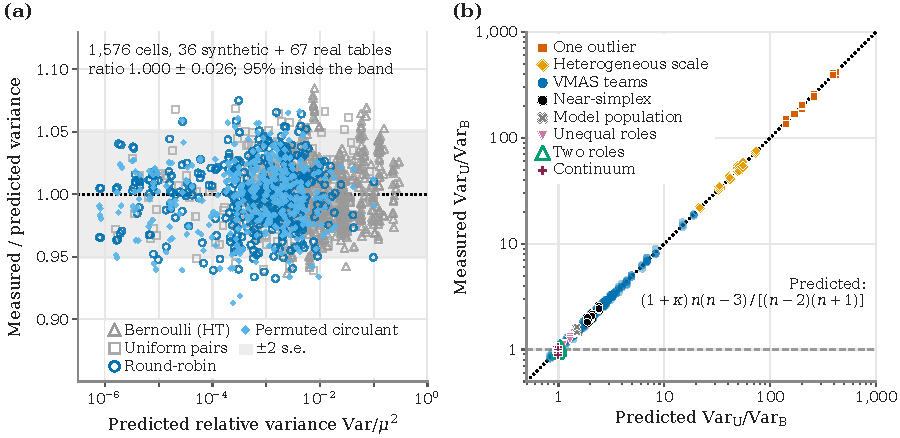
\includegraphics[width=\textwidth]{figures/fig_laws.pdf}
  \caption{\textbf{Implementation check: measured variances match the exact
  closed forms.} (a) Ratio of measured
  to predicted variance for four designs, against the predicted relative
  variance, over $1{,}576$ cells: $36$ synthetic tables and $67$ real tables
  (VMAS teams, including reset variants, and the model population), several
  degrees $k$, and $3{,}000$ draws per cell. Round-robin and permuted
  circulant are the two balanced designs. The band is $\pm2$ Monte Carlo
  standard errors of a variance estimated from $3{,}000$ draws; $95\%$ of
  the cells fall inside it, as expected if the laws are exact.
  (b) Measured versus predicted efficiency of balanced over uniform designs
  (\Cref{cor:efficiency}), from near $1$ for relational populations to
  about $140$--$420$ for a single outlier. $\mathrm{Var}_{\mathrm{U}}$ and
  $\mathrm{Var}_{\mathrm{B}}$ are the variances of the uniform and balanced
  estimates at equal $m$; the diagonal is $y=x$, and the dashed line marks
  equal efficiency.}
  \label{fig:laws}
\end{figure}



\subsection{Designs at equal cost}
\label{sec:exp-designs}

At $n=200$, \Cref{tab:e2} compares ten designs on the six synthetic
families, which isolate the failure modes predicted by
\Cref{prop:error-identity}, at a budget of $m=2n$ comparisons ($2\%$ of all pairs). Five findings stand
out, and each is a direct consequence of the anatomy.

\begin{table}[t]
\centering
\footnotesize
\setlength{\tabcolsep}{4.2pt}
\caption{\textbf{Relative error (RMSE, \%) of ten designs at equal cost.}
Synthetic populations with $n=200$; every design uses $m=2n=400$
(agent subsampling $\binom{29}{2}=406$, landmarks $397$, Bernoulli designs
in expectation; the adaptive pivot design of \citet{chechik2015average}, CCK,
spends $n-1$ comparisons on a random pivot and samples $n+1$ pairs; symmetrized nearest-neighbor graphs up to $2m$) of the
$19{,}900$ pairs ($2{,}000$ draws per cell, three tables per family; the
fixed expander is averaged over $100$ independently drawn graphs). Rows
marked $^\dagger$ are fixed structured graphs (the ring follows the generator's
ordering, by role or by angle for the last three families; the
nearest-neighbor graph is built from the table itself); their error is
pure bias, one realization per table; on the first three, exchangeable
families the ring's expected error equals the balanced design's (\Cref{thm:balanced}). ``Balanced'' is the round-robin design; HT is the Horvitz--Thompson estimator; ``unequal roles'' has
four roles of sizes $40/30/20/10\%$. Bold: within $5\%$ of the best randomized or averaged entry in the column (Monte Carlo errors below $2\%$).}
\label{tab:e2}
\begin{tabular}{@{}lcccccc@{}}
\toprule
Design & near-simplex & het.\ scale & one outlier & two roles & unequal roles & continuum \\
\midrule
Balanced & $\mathbf{0.13}$ & $0.38$ & $\mathbf{0.13}$ & $\mathbf{2.45}$ & $\mathbf{2.75}$ & $2.37$ \\
Random expander (fixed) & $\mathbf{0.13}$ & $\mathbf{0.36}$ & $\mathbf{0.13}$ & $\mathbf{2.55}$ & $\mathbf{2.82}$ & $2.42$ \\
Uniform pairs & $0.18$ & $2.14$ & $1.61$ & $\mathbf{2.49}$ & $2.91$ & $2.34$ \\
Bernoulli (ratio) & $0.18$ & $2.19$ & $1.59$ & $\mathbf{2.47}$ & $2.93$ & $2.39$ \\
Bernoulli (HT) & $4.93$ & $5.36$ & $5.17$ & $5.48$ & $5.74$ & $5.49$ \\
Agent subsampling & $0.64$ & $10$ & $7.89$ & $3.34$ & $6.26$ & $2.05$ \\
Landmarks & $1.29$ & $21$ & $15$ & $5.34$ & $12$ & $\mathbf{0.68}$ \\
Adaptive pivot (CCK) & $0.24$ & $2.20$ & $1.27$ & $3.49$ & $4.10$ & $3.53$ \\
Nearest neighbors$^\dagger$ & $7.28$ & $33$ & $8.39$ & $69$ & $90$ & $96$ \\
Fixed ring$^\dagger$ & $0.15$ & $0.32$ & $0.14$ & $46$ & $81$ & $96$ \\
\bottomrule
\end{tabular}
\end{table}

\begin{itemize}
  \item \emph{Balanced designs are the most reliable choice.} Here ``balanced'' means the randomized
  balanced design or, equivalently on average, a random regular graph
  redrawn for each estimate. Its error is the smallest, or within $1.2\times$ of
  the smallest, in five of the six families. Where individuals differ in
  distinctiveness, it beats uniform sampling by $5.7$--$12.8\times$ in error
  (ratios of unrounded values),
  that is, by $32$--$163\times$ in variance at equal cost. Where diversity is mostly relational, it nearly ties uniform
  sampling, as \Cref{cor:efficiency} predicts. The one exception is the
  continuum, where every individual has the same average distance and
  comparing everyone with a few pivots is more accurate. This exception is
  predicted by \Cref{thm:general-design}: the continuum's $\kappa=0.0008$
  lies below the threshold ${2(n-1)/\bigl(n(n-3)\bigr)}=0.010$, below which designs with
  uneven degrees have smaller variance.
  \item \emph{Horvitz--Thompson weighting, one of the Bernoulli estimators
  of Graph-SND \textup{\citep{ray2026graphsnd}}, is uniformly poor} ($4.9$--$5.7\%$).
  Its variance carries $\mu^2$ in addition to $\sigmatot$, so it cannot
  exploit any structure. The ratio form of the same design behaves like uniform
  sampling.
  \item \emph{Subsets are expensive.} Agent subsampling, which measures a
  sub-team, and landmark designs, which compare everyone to a few pivots,
  concentrate comparisons on few individuals and pay for distinctiveness
  many times over. They are $5$--$122\times$ worse in error than balanced designs
  unless diversity is mostly relational.
  \item \emph{Adaptivity does not pay at this budget.} The adaptive estimator
  of \citet{chechik2015average} samples pairs with probabilities proportional
  to distance proxies from one pivot. It is unbiased but $1.4$--$10\times$
  less accurate than the balanced design in every family, and on the real
  tables of \Cref{sec:exp-zoo,sec:exp-judge} and the VMAS teams it is
  $1.4$--$2.8\times$ less accurate than the balanced design and less
  accurate than uniform pairs, because the pivot uses half of the budget.
  \item \emph{Fixed structured graphs are unbiased only by luck.} A
  nearest-neighbor graph under-reports diversity by $7$--$96\%$, because
  it compares the most similar pairs, which have negative residuals and
over-represent the least distinctive individuals, so it suffers from both
leakage terms of \Cref{prop:error-identity}. A fixed
  ring is accurate when labels carry no information. When labels are
  ordered by role or by angle, as they often are in practice, it misses
  $46$--$96\%$ of the diversity ($46$--$81\%$ for role orderings). Randomizing the labels is what makes the guarantee of
  \Cref{thm:balanced} unconditional. A random regular graph that is drawn
  once and then fixed matches the randomized design on average over draws,
  as \Cref{thm:balanced} implies (the union-of-matchings expander of
  \Cref{tab:e2} keeps repeated edges, which raises its mean squared error by
  less than $9\%$; \Cref{app:exp-details}); its additional value is the worst-case
  guarantee of \Cref{thm:fixed-spectral}. That bound held in every case we
  tested (six families with $k\in\{4,8,16\}$ and the $1{,}024$-model population with
  $k\in\{4,8\}$), and it
  is nearly attained by rings aligned with roles or angles, whose errors come within
  $1.2$--$2.3\times$ of it, while random expanders sit at least $18\times$
  below it ($18$--$135\times$ for the closest of the $20$ graphs drawn per
  setting, $58$--$310\times$ on average).
\end{itemize}
\Cref{fig:designs} in \Cref{app:additional} shows the same qualitative picture at
five budgets from $m=n/2$ to $m=8n$. With $m=n/2$ (one comparison per
individual, $0.5\%$ of all pairs), the one-outlier population is measured
with $0.25\%$ error by the balanced design, against $3.2\%$ for uniform
pairs, $11.5\%$ for agent subsampling, and $23.5\%$ for landmarks with a
single pivot, which already uses $n-1=199$ comparisons.






\subsection{The anatomy of trained populations}
\label{sec:exp-anatomy}

We trained teams of $n\in\{8,16,32\}$ agents with independent PPO on two
VMAS tasks with different structure: Navigation, in which every agent must
reach its own goal, and Dispersion, in which all agents spawn at the center
and must consume $n$ randomly placed food particles, each once (details in
\Cref{app:exp-details:vmas}). Runs stop after $10$--$205$ iterations
(\mbox{$0.08$--$1.7$}~million environment steps) under fixed wall-clock
budgets, so they show teams early in training; seven longer runs reach
up to $766$ iterations (below).
\Cref{fig:gallery} shows two of the recorded tables
next to two synthetic references, and \Cref{fig:marl} summarizes all of them.

\begin{figure}[t]
  \centering
  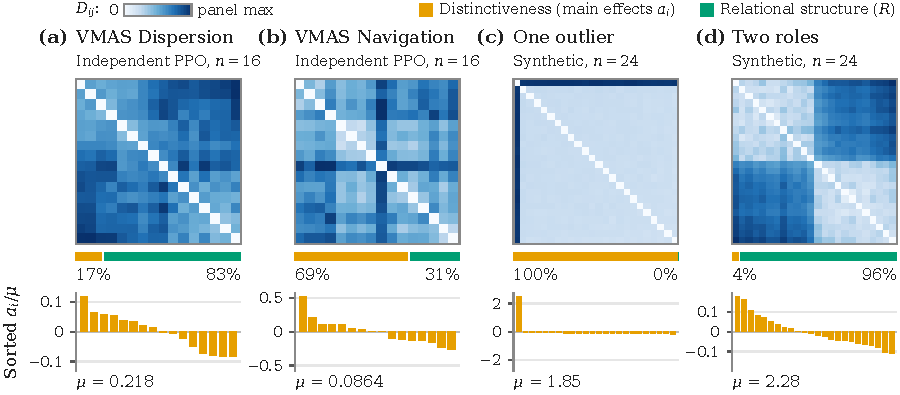
\includegraphics[width=\textwidth]{figures/fig_gallery.pdf}
  \caption{\textbf{The anatomy of diversity in four populations.} (a, b) SND
behavioral-distance tables of heterogeneous teams ($n=16$) after 41 iterations of independent PPO on VMAS Dispersion
and 35 iterations on VMAS Navigation (early in training). (c, d) Synthetic
populations generated as in Table~\ref{tab:synthetic} with $n=24$. Top: the dissimilarity table $D$, with individuals ordered by the leading eigenvector of $R$ when $R$ carries at least a quarter of the pairwise variance (a, b, d), and by distinctiveness $a_i$ otherwise (c). Each panel has its own color scale, from $0$ (white) to the panel's largest
entry (key at top left), so darker means more dissimilar. Middle: shares of the pairwise variance carried by
distinctiveness ($\sigma^2_{\mathrm{main}}/\sigma^2_{\mathrm{tot}}$, orange) and by
relational structure ($\sigma^2_{\mathrm{int}}/\sigma^2_{\mathrm{tot}}$, green), as
in Theorem~\ref{thm:anatomy}. Bottom: sorted distinctiveness $a_i/\mu$, with the level $\mu$ printed below each panel. The Dispersion
team (a) is dominated by relational structure, which varies along a single gradient rather than in blocks. The Navigation team (b) is dominated by individual distinctiveness.
Balanced designs are exact on the orange part, and their error is governed by the
green part alone (Theorem~\ref{thm:balanced}).}
\label{fig:gallery}

\end{figure}

\begin{figure}[t]
  \centering
  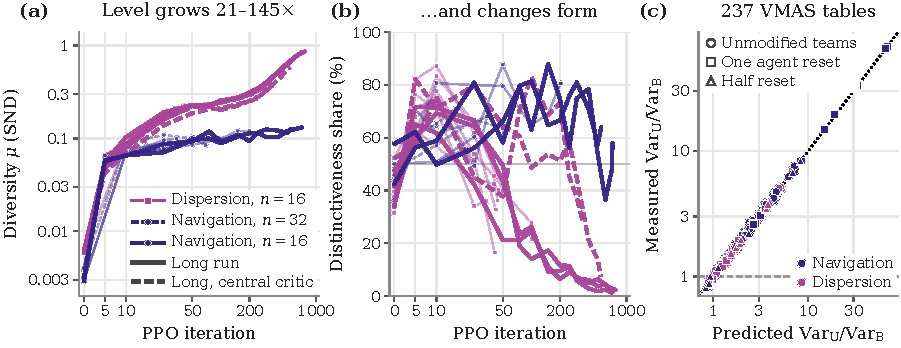
\includegraphics[width=\textwidth]{figures/fig_marl.pdf}
  \caption{\textbf{The anatomy of multi-agent teams during training.} Independent
  PPO teams on VMAS Navigation with $n=16$ (five seeds) and $n=32$ (three seeds)
  and on VMAS Dispersion with $n=16$ (six seeds); one line per seed (horizontal axis linear up to iteration $10$ and
  logarithmic beyond), each run as long as
  its compute budget allowed; bold: the seven longer $n=16$ runs
  (dashed: centralized critic). (a) Diversity $\mu$ (SND) grows by more than
  an order of magnitude from initialization.
  (b) Share of the pairwise variance carried by distinctiveness (gray line:
  $50\%$); the rest is relational. In Dispersion, which rewards agents for covering different
  targets, diversity first concentrates in individuals and then moves toward
  relational structure.
  (c) Measured ratio of uniform to balanced variance ($k=4$; $4{,}000$ draws
  each) against the prediction of \Cref{cor:efficiency} for all $237$
  VMAS tables of all runs, including the two $n=8$ Navigation runs, an
  $n=64$ initialization table, and teams with one agent or half of the
  agents reset to initialization; the median ratio of measured to
  predicted is $1.00$, and almost purely relational tables have predicted
  ratios slightly below $1$ ($0.83$--$0.99$), as \Cref{cor:efficiency} allows. Color indicates the task as in
  (a, b); dotted: $y=x$; dashed: equal efficiency.}
  \label{fig:marl}
\end{figure}

\paragraph{Diversity grows, and changes form.}
Independently initialized policies are almost interchangeable: $\mu$ is
$0.003$--$0.006$ at initialization, and distinctiveness carries $31$--$69\%$
of the pairwise variance. Training raises $\mu$ by more than an order of
magnitude, to $0.075$--$0.11$ in Navigation and $0.21$--$0.24$ in Dispersion,
but the anatomy shows that the two tasks get there differently. In all eight
Navigation runs with $n\in\{16,32\}$, distinctiveness carries $49$--$88\%$ of
the variance at every recorded iteration from iteration $5$ on and ends within
$13$ points of its maximum. In all six Dispersion runs it first rises to
$63$--$87\%$ at iterations $5$--$10$ and then falls by $23$--$62$ points, to
$17$--$40\%$, which separates the tasks without overlap (exact two-sided
permutation $p=2/\binom{14}{6}\approx7\times10^{-4}$, exploratory because we
chose the statistic after seeing the trajectories; the two noisier $n=8$
Navigation runs fall by $26$ and $30$ points, and with them $p=0.001$). Seven
longer $n=16$ runs (bold in \Cref{fig:marl}; \Cref{app:exp-details:long})
remove the difference in run length. At iteration $300$, the share is
$6$--$7\%$ in three Dispersion teams and $75$--$81\%$ in two Navigation teams;
at the end ($543$--$766$ iterations, up to $6.3$ million steps) it is $2$--$3\%$
and $58$--$64\%$, against $28$--$70\%$ for unstructured populations of
independent Gaussian points ($5$th to $95$th percentiles). Two Dispersion
teams with a centralized critic, as in MAPPO \citep{yu2022surprising}, fall
more slowly, from $76$--$82\%$ to $7$--$28\%$ after $348$--$535$ iterations.
SND alone reports only that diversity increased. We read the contrast
as a hypothesis: in Dispersion all agents spawn at one point with identical
observations, so a good team must act differently on the same input, whereas
one goal-conditioned policy solves Navigation; functional heterogeneity would
then appear as relational structure and incidental heterogeneity as
distinctiveness. Confounds remain: the observation pool changes between
iterations, and each agent's learned action standard deviation enters $W_2$.

\paragraph{Consequences for measurement.}
The predicted variance ratio of uniform to balanced designs
(\Cref{cor:efficiency}) ranges from $1.05$ to $7.1$ on these teams (an RMSE
gain of $1.02$--$2.7\times$), with median $2.4$ (interquartile range
$1.8$--$3.2$) over the $70$ tables recorded after initialization: a balanced
design typically halves the comparisons needed for a given accuracy, and the
much larger factors of \Cref{tab:e2} arise only when a few individuals
dominate distinctiveness. The ratio is largest when a few agents have drifted
far from the rest and smallest when diversity is mostly relational; in the
longer runs it reaches $7.2$ in Navigation but falls slightly below one
($0.89$--$0.99$) in late Dispersion teams, whose diversity is almost purely
relational, as \Cref{cor:efficiency} allows. For example, with $m=2n$
comparisons on one Navigation team with $n=32$, the measured relative error is
$2.16\%$ for the balanced design and $3.95\%$ for uniform pairs (predicted
$2.17\%$ and $3.90\%$), while on a late Dispersion team the two coincide
($3.01\%$ and $3.05\%$). When one agent of a team is reset to its
initialization, which mimics a failed or newly added teammate, the ratio
ranges from $1.2$ to $33$ over the $16$ teams (median $2.7$; $65$--$68$ for
the two longer Navigation runs); it is largest for the Navigation teams
trained longest and smallest for Dispersion teams ($1.2$--$1.7$, and
$0.90$--$1.8$ for the longer runs). Resetting half of a $32$-agent team,
which gives experts and novices, gives $2.1$--$8.3$; for three half-reset
Navigation teams, however, $\kappa$ is only $0.06$--$0.17$ and the ratio is
$0.83$--$0.93$ (\Cref{fig:marl}(c)), again as \Cref{cor:efficiency} allows.

\subsection{A population of trained models}
\label{sec:exp-zoo}

The theory applies to any population with a pairwise dissimilarity. As a
second domain we trained $128$ small multilayer perceptrons on
Fashion-MNIST with four training recipes ($32$ seeds each): a narrow network
trained for one epoch, a wide network trained for three epochs, the wide
network with $30\%$ label noise, and a medium network with input-noise
augmentation. Their mean test accuracies are $0.81$, $0.87$, $0.87$, and $0.86$, respectively.
The dissimilarity of two models is the Jensen--Shannon distance between
their predictive distributions, averaged over $2{,}000$ test inputs. This
distance is a pseudometric but is not separable in the sense of
\Cref{prop:separable}, so all-pairs evaluation costs
$8{,}128$ model-pair comparisons. The anatomy of this population is
${\mu=0.229}$ with a coefficient of variation of $0.51$; distinctiveness carries
$34\%$ of the pairwise variance and relational structure $66\%$. The relational part is almost
exactly low-rank: its leading eigenvector carries $86\%$ of the relational
energy and the leading three carry $98\%$. Three is the rank that four
groups produce once main effects are removed. Clustering the models by
the three leading eigenvectors of $R$ ($k$-means with four clusters)
recovers the four training recipes perfectly (adjusted Rand index $1.0$)
from the all-pairs dissimilarity table alone, without access to the recipe labels, and the
distinctiveness profile singles out the label-noise recipe as the most
distinctive (mean $a_i=+0.080$). With
$m=2n=256$ of the $8{,}128$ pairs, the measured relative error is $2.56\%$
for the balanced design (predicted $2.56\%$), $3.11\%$ for uniform pairs
(predicted $3.13\%$), and $6.98\%$ for Bernoulli sampling with the
Horvitz--Thompson estimator (predicted $6.90\%$).

The same experiment at eight times the size gives the same picture.
A population of $n=1{,}024$ models ($256$ seeds per recipe, trained in
under two minutes on one GPU) has $523{,}776$ model pairs, and its anatomy is
the same as before: $\mu=0.227$, $34\%$ distinctiveness, $66\%$ relational,
with the leading three eigenvectors of $R$ carrying $99.3\%$ of the
relational energy. With eight comparisons per model ($4{,}096$ of the
$523{,}776$ pairs),
the balanced design estimates $\mu$ to a relative error of $0.62\%$,
against $0.78\%$ for uniform pairs. At the same cost, agent subsampling,
landmarks, and a nearest-neighbor graph err by $4.2\%$, $10.4\%$, and
$65\%$, respectively. Measured variances agree with the closed-form predictions to within
Monte Carlo error at every degree tested.

% ---------------------------------------------------------------------------
% Section 5.6: neural judges and sample sets at scale.
% Every number below is in results/jmlr/samples/: judge_numbers.json, analysis_claude.json,
% claude_extra.json, claude_curve.json, analysis_opus.json (frontier generator),
% gpt5_extra.json and analysis_gpt5.json (GPT-5 judge), samples_fmnist.json.
% ---------------------------------------------------------------------------
\subsection{Neural judges and sample sets at scale}
\label{sec:exp-judge}

Some of the most expensive comparisons in current practice are made by
neural judges. Language models are widely used to judge pairs of outputs
\citep{zheng2023judging}; here a judge reads two outputs and scores how
different they are, as natural-language-inference and equivalence judges do
in diversity benchmarks \citep{stasaski2022semantic,zhang2025noveltybench}. Such a judge has no feature map, so the
all-pairs average costs at least one judge call per pair. Its scores also
need not satisfy the triangle inequality, so \Cref{thm:metric} need not
apply (although the Claude table at $T=1$ below violates none of its
$124{,}992$ triangle inequalities).
\Cref{thm:balanced}, \Cref{cor:efficiency},
\Cref{prop:sparse-anatomy,prop:rr-variance}, and the Horvitz--Thompson variance of \Cref{rem:ht-variance} do apply, because
they hold for every table, and every judge table below is symmetric by
construction. We sampled populations of $n=300$ responses from
\mbox{Qwen2.5-0.5B-Instruct} \citep{qwen2024qwen25} and
\mbox{Llama-3.2-1B-Instruct} \citep{grattafiori2024llama}. Each of $18$
populations answers one of three open-ended prompts (a one-sentence story about a robot, a name for a new coffee shop, and one sentence of advice for a first job) at temperature $T=0.5$,
$1$, or $1.5$, and three further populations mix prompts, mix generators,
or plant $2\%$ degenerate samples. Three more contain $300$ responses each
from Claude~Opus~5.5 to the same prompts, with default sampling (the API no
longer accepts a sampling temperature). A cross-encoder trained for semantic
textual similarity \citep[STS;][]{reimers2019sentence,cer2017semeval} scored every
pair in both orders, giving $d_{ij}=1-\bar s_{ij}$ with $\bar s_{ij}\in[0,1]$
the mean of the two scores. That is $89{,}700$ judge calls and $48$--$98$
GPU-seconds per population. For the first $64$ Qwen story responses at
$T=0.5$ and at $T=1$, Claude~Opus~5.5 (Anthropic) also rated all $2{,}016$
pairs from $0$ to $10$, giving $d_{ij}$ as the rating divided by $10$
(\Cref{app:exp-details:judge}).

\begin{figure}[t]
  \centering
  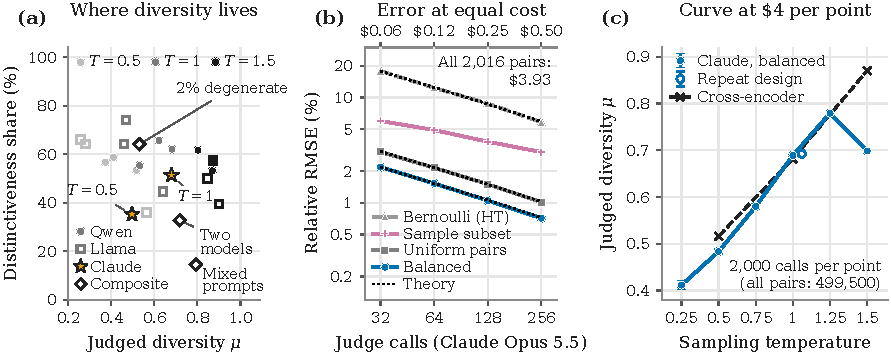
\includegraphics[width=\textwidth]{figures/fig_judge.pdf}
  \caption{\textbf{Generated text scored by neural judges.}
  (a) Judged diversity $\mu$ and the share of the pairwise variance carried
  by distinctiveness. There are $21$ cross-encoder tables with $n=300$:
  Qwen (filled circles) and Llama (open squares), shaded by sampling
  temperature, and three composite populations (diamonds). The stars are
  the first $64$ Qwen story responses at $T=0.5$ and $T=1$, judged by
  Claude~Opus~5.5 instead of the cross-encoder. (b) Relative RMSE
  against the number of Claude calls for the $64$ Qwen story responses at
  $T=1$. Colored lines and markers are measured over $4{,}000$ draws. Black
  dotted lines are the closed-form standard deviations of \Cref{thm:balanced}
  and \Cref{cor:efficiency}, and the square root of the Horvitz--Thompson
  variance of \Cref{rem:ht-variance}; the closed form of \Cref{thm:general-design} for the sample subset
  is not drawn.
  The top axis gives the API cost. (c) A diversity curve at linear cost:
  Claude-judged diversity of $1{,}000$ \mbox{Qwen2.5-0.5B-Instruct} story responses
  per temperature, each point from one randomized round-robin design with
  $k=4$ rounds ($2{,}000$ calls, about \$4; all pairs would take $499{,}500$),
  with the design-based $95\%$ interval of \Cref{prop:rr-variance} ($t$ with
  $3$ degrees of freedom), conditional on the $1{,}000$ sampled responses; except
  at $T=0.25$ the intervals are narrower than the markers. The
  open marker (offset for legibility) is an independent second design on the
  same responses. Dashed black: the exact all-pairs
  cross-encoder diversity of separate $300$-response samples from the same
  generator and prompt (another scale and sample: compare shapes).}
  \label{fig:judge}
\end{figure}

\paragraph{Where judged diversity lives.} Judged diversity rises with
temperature: for Qwen, $\mu$ ranges over $0.37$--$0.52$ at $T=0.5$ and
$0.80$--$0.87$ at $T=1.5$. Its anatomy, however, shows no consistent trend
with temperature. For a single prompt and a small generator scored by the cross-encoder,
distinctiveness carries $36$--$74\%$
of the pairwise variance (\Cref{fig:judge}(a)), because individual samples
differ in how far they sit from all others, and the anatomy names them. At
$T=0.5$, the three least distinctive of the $300$ samples under the
cross-encoder are variants of one template (``A sleek humanoid robot named
Echo\ldots''), and two of the three least distinctive of the $64$ under
Claude are Echo variants as well. At $T=1$, the two most distinctive samples under Claude are a
response that switched to Chinese and an off-topic hacker story. Under the
cross-encoder, on the same $64$ responses, the hacker story ranks first and
the Chinese response third; on all $300$, a ``Lorem ipsum'' passage also
enters the top three. Planting six degenerate samples among $300$ raises the
distinctiveness share from $53\%$ to $64\%$. Mixing the three prompts at
$T=1$ lowers it from $55$--$66\%$ to $15\%$, because the prompts act as
roles and the structure becomes relational.

\paragraph{Frontier models as generators and as judges.} Responses from a
frontier model are far less diverse under this judge, as other measures
also find \citep{zhang2025noveltybench,jiang2025hivemind}. (The contrast is
descriptive: the open models were capped at $40$ new tokens, so $66$--$100\%$ of
their responses end mid-sentence, whereas the API model's are complete.) For the Claude~Opus~5.5 populations, $\mu$ is
only $0.22$--$0.41$, below every Qwen population at $T=1$
($0.53$--$0.68$). The anatomy separates coffee-shop names that fall into a
few modes ($17\%$ distinctiveness, so mostly relational) from advice that
repeats one template with idiosyncratic exceptions ($69\%$). The closed
forms hold here as well; for example, the story prompt at $m=2n$ gives
$0.89\%$ error against $0.89\%$ predicted, and single-design intervals cover
$\mu$ in $94.6$--$95.9\%$ of draws. Claude and the cross-encoder score on different scales (a rating divided
by $10$ against one minus an STS probability), so we compare them by rank:
they correlate $0.54$--$0.68$ pair by pair, and their distinctiveness
rankings of the $64$ responses have Spearman correlations of $0.53$ ($T=1$)
and $0.80$ ($T=0.5$). A third judge from another vendor, GPT-5 (OpenAI),
scored the same $2{,}016$ pairs at $T=1$. It gives $\mu=0.682$, correlates
$0.64$ with Claude pair by pair (Claude's own order-swapped retest gives
$0.74$), and ranks the $64$ responses by distinctiveness with a Spearman
correlation of $0.86$ against Claude, with the same two responses on top.
The closed forms hold on its table too ($0.89\%$ error at $m=2n$ against
$0.90\%$ predicted).

\paragraph{Fewer judge calls, with error bars.} Here the estimand is
the diversity of the sampled responses, and errors refer to the design;
claims about a generator add the sampling variance $4\zeta_1/n+O(n^{-2})$
(\Cref{sec:discussion}). Claude's order-swapped retest puts call noise at up
to $46\%$ of $\sigmaint$ ($T=1$), and $97\%$ of such noise is relational, so
$\kappa=1.05$ is attenuated (about $1.9$ without it). Because distinctiveness
carries much of the variance ($\kappa=0.56$--$2.85$), \Cref{cor:efficiency} predicts
that uniform pair sampling needs $1.6$--$3.8$ times as many judge calls as a
balanced design on the Qwen and Llama single-prompt populations, and the
measurements agree ($4{,}000$ design draws per cell). With $m=2n$ pairs, the
relative error on the Qwen story population at $T=1$ is $0.49\%$ for the
balanced design (predicted $0.48\%$) and $0.77\%$ for uniform pairs
(predicted $0.78\%$). It is $4.1\%$ for Bernoulli sampling with the
Horvitz--Thompson estimator, and $3.4\%$ for all pairs among a random subset
of samples, the most common shortcut. With Claude as the judge on the $T=1$
population (\Cref{fig:judge}(b)), $128$ calls cost about $\$0.25$, against
$\$3.93$ for all pairs, and give $1.05\%$ error (predicted $1.07\%$);
uniform pairs give $1.51\%$ (predicted $1.50\%$). On the less diverse
$T=0.5$ population, the same $128$ calls give $1.87\%$ (predicted $1.90\%$)
against $2.33\%$ for uniform pairs. Over all $276$ combinations of the $23$ tables of \Cref{fig:judge}(a) ($21$ cross-encoder and $2$ Claude-judged),
the three designs with a closed form, and the budgets $m\in\{n/2,n,2n,4n\}$ ($4{,}000$ draws each), the ratio of measured to predicted
variance has median $0.999$, and $90\%$ of the ratios lie in $[0.96,1.04]$.
A single round-robin design with $k\in\{4,8\}$ gives a
$95\%$ interval (\Cref{sec:exp-ci}) that covers $\mu$ in $94.5$--$95.7\%$ of
draws on every table of \Cref{fig:judge}. On the single-prompt populations of \Cref{fig:judge}(a), the same $m=2n$ pairs
rank samples by distinctiveness with a median Spearman correlation of
$0.61$--$0.82$ against the all-pairs ranking ($0.49$ on the three-prompt
mixture).

\paragraph{A curve that all pairs cannot afford.} Linear cost also makes
analyses possible that the all-pairs average prices out. For $1{,}000$ story
responses at each of six temperatures, all pairs would take $499{,}500$
Claude calls per temperature, about \$1{,}000. One round-robin design with
$k=4$ rounds takes $2{,}000$ calls (about \$4), and through
\Cref{prop:rr-variance} it comes with its own error bar. \Cref{fig:judge}(c)
shows the result. Judged diversity rises from $0.411$ at $T=0.25$ to $0.779$
at $T=1.25$, with $95\%$ interval half-widths of $0.4$--$2.3\%$ of $\widehat\mu$. It then falls to
$0.698$ at $T=1.5$, where most responses degenerate into mixed-language
noise and Claude rates pairs of them as less different from each other. The
cross-encoder instead rates such noise as the most diverse ($\mu=0.870$ at
$T=1.5$). Which notion of
diversity is wanted is a modeling choice. The point here is that the cheap
estimate is accurate enough to reveal the difference, for about \$29
in total, including a repeat design at $T=1$, instead of about \$6{,}000 for
all pairs at the six temperatures. The same calls also flag failures: at each
temperature from $0.5$ to $1$, the response with the largest estimated
distinctiveness $\widehat a_i$ (\Cref{prop:sparse-anatomy}) is a refusal such
as ``I'm sorry, but I can't assist with that.'' The independent repeat design
at $T=1$ gave $0.692$ (interval $[0.689,0.696]$, against $[0.686,0.691]$ for
the first). The difference, $0.0035$, is $2.5$ standard errors when each
design's own variance estimate is used; with $k=4$ rounds these estimates
have only $3$ degrees of freedom (coefficient of variation about $40\%$), so
the intervals are approximate, and more rounds give steadier error bars.

\paragraph{Sample sets at scale and the Vendi score.} On $60{,}000$
Fashion-MNIST images \citep{xiao2017fashion}, compared by the Euclidean
distance between features of a small trained classifier, $m=n/2=30{,}000$
comparisons ($0.0017\%$ of the $1.8\times10^9$ pairs; $1{,}000$ draws) give
$0.169\%$ error (predicted $0.167\%$). Uniform pairs give $0.207\%$,
Bernoulli sampling $0.59\%$, and a subset of samples $1.96\%$. The order-$2$
Vendi score \citep{friedman2023vendi,pasarkar2024cousins}, which equals the
R\'enyi-kernel-entropy mode count of \citet{jalali2023information}, is
$\mathrm{VS}_2=n/\bigl(1+(n-1)\,\bar q\bigr)$, where $\bar q$ is the average
of $q_{ij}=s_{ij}^2$ for a similarity kernel with $s_{ii}=1$. It is therefore a pairwise
average in disguise, and the same comparisons estimate $\bar q$ without bias
(the plug-in $\mathrm{VS}_2$, convex in $\bar q$, is biased slightly upward). With a Gaussian
kernel, the error is $0.29\%$ for the balanced design, $0.34\%$ for uniform
pairs, and $2.9\%$ for a subset. On text, with the judge's similarity as the
kernel (not necessarily positive semidefinite, so $\mathrm{VS}_2$ is then defined
by the formula above), the error at $m=2n$ is $2.1\%$ for the balanced design against
$3.0\%$ for uniform pairs (cross-encoder, Qwen story population at $T=1$),
and $4.1\%$ against $5.6\%$ (Claude, $T=1$). With the cross-encoder's similarity as the
kernel, $\mathrm{VS}_2$ is $1.6$--$2.7$ for each set of $300$ frontier-model
responses, against $4.2$--$8.3$ for Qwen at $T=1$. Because this kernel gives
substantial similarity to any two on-topic texts (a constant similarity $s$
gives $\mathrm{VS}_2\approx1/s^2$ whatever the content), these values rank
populations under one kernel rather than count distinct responses. For kernels with an explicit
low-dimensional feature map, exact computation is already inexpensive. The
gain is for implicit kernels and judges: at $n=10{,}000$, all pairs would
take $5\times10^7$ judge calls, and a balanced design with $m=2n$ takes
$2\times10^4$.


\subsection{Error bars and the anatomy from the same comparisons}
\label{sec:exp-ci}

The round-robin design (\Cref{sec:balanced}) also provides an error
bar and the anatomy without extra comparisons. For even $n$, a round-robin schedule applied after a
uniform relabeling partitions all $N$ pairs into $n-1$ rounds of $n/2$
disjoint pairs, so the
round means average exactly to $\mu$. Choosing the $k$ rounds at random
makes their means a simple random sample from these $n-1$ values, and a
$t$-interval over the $k$ round means with the finite-population correction
$1-k/(n-1)$ is the classical random-group interval \citep{wolter2007introduction}:
its variance estimate is exactly unbiased (\Cref{prop:rr-variance}), and its
coverage rests on approximate normality of the round means \citep{hajek1960limiting}. Over $26$ tables (six synthetic
families, the model population, and $19$ VMAS tables: four trained teams
and $14$ reset variants from seven of the first nine training runs,
plus one untrained $n=100$ team; $2{,}000$
draws per table), this interval covers $\mu$ in $95.0$--$95.2\%$ of draws at the
nominal $95\%$ level for $k\in\{2,4,8,16\}$, and every table lies between
$93.6\%$ and $96.4\%$ (at $k=16$, only the $13$ tables with $n\ge 32$ admit
the design). The usual Wald interval for uniform pairs
undercovers on populations with an outlier ($88.3\%$ at $k=2$). At $k=4$
the balanced interval on the one-outlier table is $8\times$ narrower than the Wald interval
($0.72\%$ of $\mu$ against $5.93\%$). With $k=2$ the $t$-quantile on one
degree of freedom makes intervals wide, and on the three $n=64$ judge tables
of \Cref{sec:exp-judge} they also undercover slightly ($91.9$--$94.1\%$), so
we recommend $k\ge4$ when error bars are needed. The same comparisons also rank individuals by
distinctiveness (\Cref{prop:sparse-anatomy}). On these $19$ VMAS tables,
the Spearman correlation between $\widehat a$ and $a$ (over the first $300$
draws per table) is $0.74$ with four comparisons per agent and $0.91$ with
sixteen (on the six tables with $n\ge32$; \Cref{fig:ci} in
\Cref{app:additional}).

\subsection{Closed-loop diversity control}
\label{sec:exp-control}

\Cref{prop:dico} predicts that a diversity controller driven by a sparse
estimate tracks its target with relative error $-e/(1+e)$, where $e$ is the
estimator's relative error, so to first order the tracking error is the
estimation error with its sign reversed. We
test this in two ways: a controlled simulation that isolates the
mechanism, and DiCo training runs in VMAS.

\paragraph{Simulated control with drifting policies (no learning).}
A DiCo-style controller rescales the agent-specific action components of
$n$ agents by the factor $c_t=\SNDdes/\widehat\mu_t$ at every step, while the components
follow a random drift between steps. The distance is the mean Euclidean
distance between agent-specific action means over a batch of $32$
observations, which is $W_2$ for Gaussians with a shared covariance and is
homogeneous of degree one, so the realized diversity equals
$\SNDdes\,\mu_t/\widehat\mu_t$ identically. The simulation therefore shows
how each design's estimation error becomes tracking error as the population
drifts; it does not model learning. We run $300$ steps for teams with
equal agent scales (homogeneous teams, $\kappa=0.10$--$0.24$) and heterogeneous teams, whose agents differ
in scale ($\kappa=8$--$31$), at $n=50$ with $m=125$ comparisons per step
(round-robin, $k=5$) and at $n=500$ with $m=2{,}000$ of $124{,}750$ pairs
($k=8$), on $10$ independently drawn populations per setting
(\Cref{app:exp-details:sim-control}).
\Cref{fig:control} shows that every measured tracking error matches its
first-order prediction. For heterogeneous teams at $n=500$, the
root-mean-square tracking error is $0.320\pm0.004\%$ with the balanced
design (predicted $0.318\%$), $1.42\pm0.05\%$ with uniform pairs (predicted
$1.41\%$), $1.39\pm0.04\%$ with Bernoulli sampling and the ratio estimator (first-order
lower bound $1.41\%$, met within Monte Carlo error),
and $2.63\pm0.05\%$ with the Horvitz--Thompson estimator (predicted
$2.63\%$). For heterogeneous teams at $n=50$ the balanced design cuts the error from $5.3\%$ (uniform pairs) to
$1.23\%$, a factor of $4.3$. With homogeneous scales, balanced and uniform
designs perform alike ($1.27\%$ versus $1.40\%$ at $n=50$, and $0.344\%$
versus $0.364\%$ at $n=500$), as \Cref{cor:efficiency} predicts. Where the
estimation error is large, the mean tracking error is positive and close to
the mean squared estimation error, which is the second-order bias of
\Cref{prop:dico}. For heterogeneous teams
at $n=50$ it is ${+0.98\pm0.23\%}$ with Horvitz--Thompson weighting (squared
RMSE $1.05\%$), ${+0.33\pm0.14\%}$ with uniform pairs ($0.28\%$), and
$+0.02\pm0.02\%$ with the balanced design ($0.015\%$).

\begin{figure}[t]
  \centering
  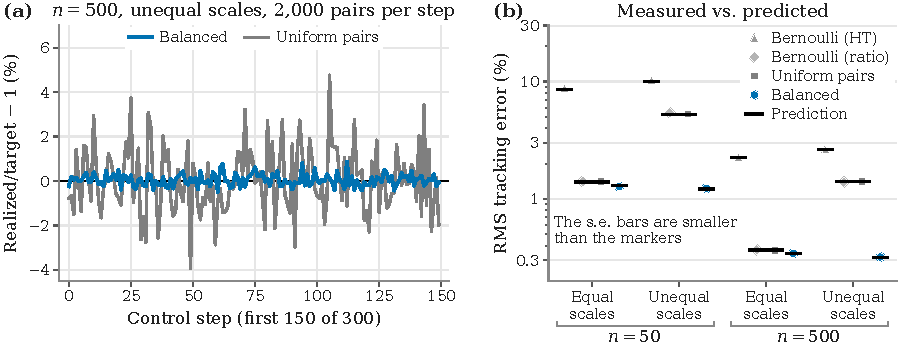
\includegraphics[width=\textwidth]{figures/fig_control.pdf}
  \caption{\textbf{A diversity controller inherits the estimator's error,
  and balanced designs shrink it.} (a) Realized diversity relative to the
  target for a DiCo-style controller on a $500$-agent team whose agents
  differ in scale, using $2{,}000$ comparisons per step ($1.6\%$ of all
  pairs); first $150$ of $300$ steps of one population. (b) Root-mean-square
  tracking error over $300$ steps for teams of $n=50$ or $500$ agents with
  equal or unequal scales, mean $\pm$ standard error over $10$ populations
  per setting. Short black bars through the markers are first-order predictions (the
  RMS of the relative estimation error $e$) from \Cref{thm:balanced}
  (balanced), \Cref{cor:efficiency} (uniform pairs; for the Bernoulli ratio
  estimator, the uniform-pairs value at $m=pN$, a first-order lower bound), and
  \Cref{rem:ht-variance} (Horvitz--Thompson);
  \Cref{prop:dico} maps $e$ to the tracking error $-e/(1+e)$. In this
  simulation, all-pairs control has zero error by construction.}
  \label{fig:control}
\end{figure}

\paragraph{DiCo in multi-agent reinforcement learning.}
We next replace the all-pairs SND inside DiCo \citep{bettini2024dico} with a
sparse estimate and train teams of $n=50$ agents with independent PPO on
VMAS Dispersion for $167$ iterations, at the set points
$\SNDdes\in\{0.12,0.14,0.15\}$ with three seeds each. Every cell is trained
with all-pairs SND, with Bernoulli sampling at $p=0.1$ and the ratio
estimator ($122.5$ of $1{,}225$ pairs per call in expectation), and, at the
two lower set points, with the randomized balanced design: a fresh random
$5$-regular comparison graph at every call ($125$ pairs; \Cref{thm:balanced}).
By Jensen's inequality and \Cref{cor:efficiency}, Bernoulli sampling is per
call at least $0.96\,(1+\kappa)$ times as variable as the balanced design. The Bernoulli and
all-pairs runs of a cell share seeds and environment initializations, so
their rollouts diverge only once the estimates differ; the balanced runs
reuse the seeds on a later software stack with evaluation rollouts disabled,
on which two all-pairs runs reproduce the earlier ones to within seed-to-seed
variation (\Cref{app:exp-details:dico}), so comparisons with them match cells
by seed and set point only and include any stack effect. The DiCo
distance is homogeneous of degree one, so \Cref{prop:dico} applies
(\Cref{app:exp-details:dico}).

\Cref{tab:dico} reports the final $50$ iterations. An all-pairs audit of
the controlled policies, never fed back to the controller, finds their
seed-averaged realized SND within $0.51\%$ of both targets with the
balanced design (at most $0.57\%$ for a single seed), against $0.61\%$
($0.71\%$) with Bernoulli sampling and $0.48\%$ ($0.54\%$) with all-pairs
control at the same set points. We
detect no change in reward, but three seeds give little power. The set
points of one seed share initial conditions, and their reward differences
are strongly correlated, so we treat seeds as the unit: the mean reward per
step differs from all-pairs control by $(4.6\pm12.5)\times10^{-3}$ with
Bernoulli sampling and by $(9.1\pm11.4)\times10^{-3}$ with the balanced
design (mean $\pm$ standard error over three seeds; $t=0.37$ and $0.80$ on
two degrees of freedom), and the $95\%$ intervals exclude only differences
beyond about $-15\%$ and $+18\%$ of the mean reward. The two sparse designs
differ by $(1.1\pm4.1)\times10^{-3}$ in reward (interval within $\pm6\%$)
and by $-0.08\pm0.10$ percentage points in audit error
(per-cell values in \Cref{tab:dico-cells}). These runs show that sparse estimation can replace all-pairs SND in DiCo
without detectable loss, not that the choice of design matters in closed
loop: with DiCo's soft update added to the simulation above
(\Cref{tab:tau}), the balanced design's $4.0\times$ smaller tracking error at
$\tau=1$ ($n=50$, unequal scales) shrinks to $2.4\times$ at $\tau=0.1$ and
vanishes at $\tau\le0.03$, where the lag of the running average dominates
every design, all pairs included. The
metric cost per call falls $9.3$--$9.6\times$ with Bernoulli sampling
($19.7$ to $2.1$\,ms on an RTX~4090) and $8.5$--$9.0\times$ with the
balanced design (\mbox{$196$--$205$} to $23$\,ms on a shared Quadro RTX~5000),
close to the $10\times$ and $9.8\times$ reductions in pairs. These times are for
the reference DiCo implementation, which loops over pairs; a vectorized
all-pairs computation takes about $0.6$\,ms at this $n$ (\Cref{fig:scale}),
so in MARL, sparse designs pay off with thousands of policies or with
rollout-based comparisons.

\begin{table}[t]
\centering
\small
\caption{\textbf{DiCo with a sparse SND estimate: no detectable loss against all pairs.}
($n=50$ agents, VMAS Dispersion, three seeds per set point, final $50$ of $167$
iterations). Balanced: a fresh random $5$-regular comparison graph at every
call ($125$ of $1{,}225$ pairs); Bernoulli: $p=0.1$ ($122.5$ pairs in
expectation). Audit error: relative deviation of the realized all-pairs SND
from the target, measured on $4{,}096$ observations of each iteration's
rollouts before they are used for training, and never fed back; all-pairs control also errs, because DiCo rescales with a running
average ($\tau=0.01$) of per-batch SND values. Reward: mean reward per step over the training batches,
with its standard error over seeds. Balanced runs cover the two lower set
points.}
\label{tab:dico}
\begin{tabular}{@{}ccccccc@{}}
\toprule
& \multicolumn{3}{c}{Audit error (\%)} & \multicolumn{3}{c}{Reward} \\
\cmidrule(lr){2-4}\cmidrule(l){5-7}
$\SNDdes$ & balanced & Bernoulli & all pairs & balanced & Bernoulli & all pairs \\
\midrule
$0.12$ & $0.44$ & $0.50$ & $0.48$ & $0.307\pm0.008$ & $0.316\pm0.008$ & $0.306\pm0.004$ \\
$0.14$ & $0.51$ & $0.61$ & $0.36$ & $0.346\pm0.002$ & $0.335\pm0.006$ & $0.329\pm0.012$ \\
$0.15$ & -- & $0.43$ & $0.46$ & -- & $0.339\pm0.011$ & $0.3412\pm0.0004$ \\
\bottomrule
\end{tabular}
\end{table}



\subsection{Cost at scale}
\label{sec:exp-scale}

\Cref{fig:scale}(a) reports the wall-clock time of one complete diversity
evaluation, including the forward passes of all $n$ policies on a shared
batch of $1{,}024$ observations, on a single RTX~3080 GPU. All-pairs SND
grows quadratically, from $0.6$\,ms at $n=50$ to $3.1$\,s at $n=5{,}000$.
The balanced design grows linearly: at $n=5{,}000$ and $k=8$ it takes
$24$\,ms, which is $131\times$ faster (below the $625\times$ ratio of pair
counts, because both include the forward passes of all $n$ policies), and
$48$\,ms at $n=10{,}000$. \Cref{fig:scale}(b) shows that accuracy improves
at the same time. With $k$ fixed, the relative standard deviation of the
balanced estimate falls with $n$, to $0.054\%$ at $n=5{,}000$ and $k=8$
(predicted $0.054\%$), because the relative variance is about
$2\sigmaint/(\mu^2nk)$ (\Cref{thm:balanced}) and at most $v_{n,k}<2/(nk)$
for every metric (\Cref{thm:metric}); the latter bound is loose here because
independently initialized policies are nearly equidistant.

\begin{figure}[!t]
  \centering
  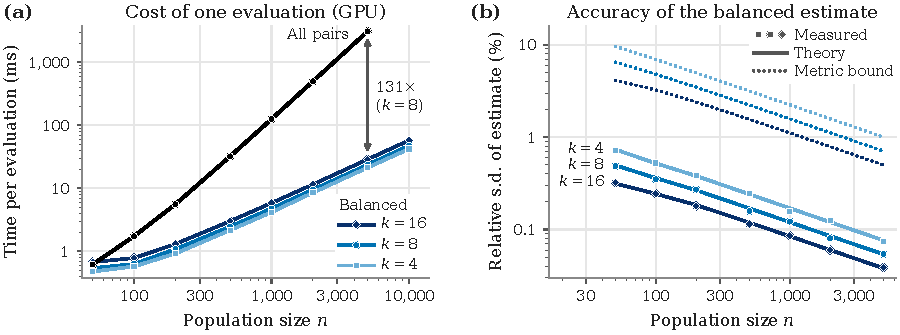
\includegraphics[width=\textwidth]{figures/fig_scale.pdf}
  \caption{\textbf{Linear cost and improving accuracy at scale.} (a) Wall-clock
  time of one SND evaluation for $n$ independently initialized Gaussian
  policies (median of repeated calls, RTX~3080). All pairs are measured up
  to $n=5{,}000$; the arrow marks the $131\times$ speedup of the balanced
  design with $k=8$ at $n=5{,}000$. (b) Relative standard deviation of the
  balanced estimate over $400$ independent designs (markers: squares,
  circles, and diamonds for $k=4$, $8$, and $16$; Monte Carlo standard errors
  are smaller than the markers), the closed-form prediction of
  \Cref{thm:balanced} computed from the full table (solid lines), and the
  metric-universal bound $\sqrt{v_{n,k}}$ of \Cref{thm:metric} (dotted).}
  \label{fig:scale}
\end{figure}




% ======================================================================
% ============================================================
% related_work.tex -- natbib author-year; all keys are in refs.bib
% ============================================================
\section{Related Work}
\label{sec:related}

\paragraph{Diversity as a mean pairwise dissimilarity.}
The average dissimilarity over all pairs of a population is one of the oldest
and most widely used diversity statistics in science. Up to a factor $(n-1)/n$, it is Rao's quadratic
entropy in ecology \citep{rao1982diversity}. Effective-number transformations
of it and of related similarity-sensitive indices are standard there
\citep{hill1973diversity,leinster2012measuring,chiu2014distance}. In population
genetics, nucleotide diversity is the mean number of pairwise sequence
differences \citep{nei1979mathematical,tajima1983evolutionary}. Machine learning
uses the same functional, or close relatives of it, throughout. It appears as
disagreement-based ensemble diversity \citep{kuncheva2003measures}, Self-BLEU for
generated text (an average of multi-reference BLEU scores; \citealp{zhu2018texygen}),
the average learned sentence similarity between pairs of responses
\citep{tevet2021evaluating},
and mean pairwise perceptual (LPIPS) distance for generated images
\citep{zhu2017toward,zhang2018unreasonable}, whose standard protocol already
averages only $19$ consecutive pairs of $20$ samples, a sparse design of the
kind analyzed here. It also appears as internal diversity of
generated molecules \citep{polykovskiy2020molecular}, as the output diversity of
aligned language models \citep{kirk2024understanding}, and as the diversity
coefficient of training data \citep{miranda2023beyond}. For $n$ equally weighted
regression members, the ambiguity term of the squared-loss ensemble
decomposition \citep{krogh1995neural} is $(n-1)/(2n)$ times the mean pairwise
squared distance between their predictions, and \citet{wood2023unified} extend
this diversity term to bias-variance-diversity decompositions of other losses. Kernel-based
effective-number scores such as the Vendi score \citep{friedman2023vendi} are
not pair averages in general. Their order-$2$ members \citep{pasarkar2024cousins},
however, are monotone
functions of a mean pairwise (squared) similarity, with the diagonal included, so
the designs of \Cref{sec:designs} also cover them (\Cref{sec:exp-judge}). The order-$2$ R\'enyi kernel
entropy of \citet{jalali2023information} is one such member, and
\citet{ospanov2024scalable} approximate it and the Vendi score in linear time
with random Fourier features, which requires a shift-invariant kernel on
explicit inputs. In MARL, the same average is SND \citep{bettini2025snd}. Except for Self-BLEU and Vendi scores of order other than~$2$, each of these
statistics is a complete degree-two U-statistic over the population or a
monotone function of one. When each comparison
is expensive, as with rollouts, Wasserstein distances over many states, or
judge-based comparisons \citep{zheng2023judging}, its $\binom{n}{2}$ cost becomes the bottleneck that
this paper removes.

\paragraph{Behavioral diversity and heterogeneity in MARL.}
Diversity in MARL has been quantified through policy and joint-action
distributions \citep{yu2021informative,mckee2022diversity,hu2022policy},
occupancy measures \citep{liu2021unifying}, trajectory distributions
\citep{lupu2021trajedi}, population determinants
\citep{parker-holder2020effective}, and robotic heterogeneity indices
\citep{balch2000hse,twu2014measure,prorok2017impact}. A complementary line of
work learns heterogeneous behavior through selective or masked parameter
sharing \citep{christianos2021scaling,li2024kaleidoscope}, diversity
regularization \citep{li2021celebrating}, roles
\citep{wang2020roma,wang2021rode}, heterogeneous graph policies
\citep{bettini2023hetgppo}, and hypernetworks \citep{tessera2024hypermarl};
pairwise policy distances serve as diagnostics \citep{hu2024measuring}, and
per-agent parameters are now standard \citep{zhong2024heterogeneous}. SND is
widely used in this line: DiCo holds it at a set point
\citep{bettini2024dico}, it is used to study when heterogeneity pays off
\citep{bettini2024impact,amir2025diversity}, and DiCo-style control has
group-aware and extremum-seeking variants
\citep{yang2025structured,patel2026optimizing}. Identity-free alternatives
address agents that swap roles \citep{buchi2026events}, and diversity is
also studied in societies of language-model agents \citep{huot2026routing}.
All of these pairwise measures evaluate every pair of agents. Our designs
evaluate linearly many pairs with exact guarantees, and the anatomy adds a
per-agent and relational reading of the same quantity
(\Cref{sec:exp-anatomy}).

\paragraph{Incomplete U-statistics and design of comparisons.}
Averages of a degree-two kernel over a subset of pairs are incomplete
U-statistics \citep{blom1976some}. Classical work mostly treats the data as i.i.d.\
draws and studies the variance about the population parameter.
\citet{blom1976some} and \citet{lee1982incomplete} give the exact
variance of an incomplete U\nobreakdash-statistic in terms of how many selected
pairs share an observation, so for a degree-two kernel a design enters only
through its degree sequence. For a non-degenerate kernel, designs in which every
observation appears equally often recover the efficiency of the complete
statistic once the number of pairs grows faster than $n$
\citep{brown1978reduced,lee1982incomplete,lee1990ustatistics}, and designs
built from orthogonal arrays can be asymptotically efficient even when it grows
more slowly than $n$ \citep{kong2021design}. Recently,
\citet{miglioli2025incomplete} gave efficient algorithms for constructing
equireplicate designs and proved a Berry--Esseen bound for incomplete
U-statistics of deterministic designs that also covers degenerate kernels. Random designs were analyzed by
\citet{janson1984asymptotic} and, conditionally on the data and in high dimensions, by
\citet{chen2019randomized}. Incomplete
U-statistics scale empirical risk minimization through randomly sampled tuples
\citep{clemencon2016scaling} and kernel two-sample testing through fixed
designs, from the linear-time maximum mean discrepancy (MMD) over disjoint pairs \citep{gretton2012kernel}
to aggregated tests whose cost interpolates between linear and quadratic time
\citep{schrab2022efficient}.
Balanced sampling in survey statistics selects random samples, with
prescribed inclusion probabilities, whose Horvitz\nobreakdash--Thompson
estimates of the totals of auxiliary variables equal the known population
totals \citep{deville2004efficient}. In that
terminology, our balanced designs are balanced samples of pairs with respect to
the $n$ individual-incidence variables, and \Cref{thm:balanced} gives their exact
variance, which for general balanced samples is only approximated
\citep{deville2005variance}. Horvitz\nobreakdash--Thompson weighting
\citep{horvitz1952generalization} underlies the Bernoulli designs used as
baselines.

\paragraph{What changes for a fixed population.}
In our setting the population of $n$ agents or models is fixed and, as in the
finite-population theory of U-statistics
\citep{nandi1963properties,bloznelis2001orthogonal}, the target is the
complete statistic itself rather than a superpopulation mean. Much of the
classical machinery carries over (\Cref{rem:classical}). A regular design
removes the main effects in every realization, just as, for i.i.d.\ data, it has
the same H\'ajek projection as the complete statistic, and the variance of a relabeled design is
a permutation moment of a quadratic-assignment (Mantel) statistic
\citep{daniels1944relation,mantel1967detection,hubert1976quadratic,hubert1987assignment},
which \Cref{thm:general-design} expresses through the anatomy. Two things
change. First, the benchmark changes: classical efficiency is measured against the
sampling error of the complete statistic about the population parameter, and
against that benchmark fewer than $n$ evaluations can suffice
\citep{kong2021design}, whereas estimating the complete statistic of a fixed
population needs $\Omega(n)$ evaluations (\Cref{prop:lower}, whose
constructions follow \citealp{barhum2007approximating}). Second, the
finite-population correction, which disappears over an i.i.d.\ superpopulation
(\Cref{rem:classical}), lets irregular designs such as landmarks do better when
$\kappa<2(n-1)/\bigl(n(n-3)\bigr)$. The normal limit of quadratic-assignment
statistics \citep{barbour1986random} justifies approximate intervals. When item parameters are estimated from pairwise comparisons, the topology of
the comparison graph governs the minimax rate \citep{shah2016estimation}.

\paragraph{Sublinear estimation of average distance.}
In sublinear algorithms, \citet{indyk1999sublinear} showed that the average
distance of $n$ points in a metric space can be approximated within a factor $1\pm\varepsilon$
using $O(n/\varepsilon^{7/2})$ distance queries.
\citet{barhum2007approximating} showed that $O(n/\varepsilon^2)$ uniformly
sampled pairs suffice, which is tight for uniform sampling.
\citet{chechik2015average} reached $O(n+\varepsilon^{-2})$ queries with unbiased
estimates built from a weighted sample of pairs, whose construction itself uses
$O(n)$ distance computations. \citet{chang2017metric} analyzed a uniformly
random perfect matching, our design with $k=1$, for the metric 1-median
problem; his variance bound needs a diameter condition
\citep[see also][]{chang2022random} that he verifies for graph metrics, where it gives $(1\pm\varepsilon)$ estimates of the average
distance, while for general metrics he obtains one-sided constant-factor
estimates. \Cref{thm:metric} with $k=1$ makes a single random perfect
matching a two-sided $(1\pm\sqrt{8/n})$-approximation with probability at
least $3/4$ for every pseudometric. Related average-parameter problems for graphs are
treated by \citet{feige2006sums} and \citet{goldreich2008approximating}. Answering a
question of \citet{mendel2015expanders}, \citet{eskenazis2026optimal} give a
deterministic algorithm that queries $O(n)$ distances and approximates the average
distance of a typical regular graph within a constant factor; they also show that no
deterministic algorithm with $O(n)$ queries achieves a constant factor for all
bounded-degree graphs. For several positive-definite kernels on
Euclidean inputs, including the Gaussian kernel, the sum of all kernel entries, and hence a mean pairwise
similarity, can be estimated in time sublinear in $n$ by kernel density
estimation \citep{backurs2021faster}. That approach needs explicit inputs and
positive definiteness. With only a dissimilarity oracle, $\Omega(n+\varepsilon^{-2})$
evaluations are necessary (\Cref{prop:lower}). For constant failure
probability, \Cref{thm:metric} attains this budget with a design that is
non-adaptive and uniformly weighted and whose variance is known in closed
form for every table. For failure probability $\eta$, the adaptive scheme
needs only $O(n+\varepsilon^{-2}\log(1/\eta))$ evaluations
\citep[Theorem~1.3]{chechik2015average}, whereas the median of balanced
designs pays the factor $\log(1/\eta)$ on the $n$ term as well.

\paragraph{Decompositions of dyadic data.}
The anatomy is the two-way analysis of variance of a symmetric dyadic table,
which in plant breeding is Griffing's diallel analysis of general and specific
combining ability \citep{griffing1956concept}. It coincides with the
finite-population Hoeffding decomposition of a degree-two U-statistic
\citep{nandi1963properties,bloznelis2001orthogonal}, with the symmetric social relations model for
interpersonal data \citep{kenny1984social}, and with the spectral analysis of
data on two-element subsets through the representation theory of the symmetric
group \citep{james1978representation,diaconis1988group}. Related double-centering
operations underlie classical multidimensional scaling
\citep{torgerson1952multidimensional,gower1966some} and distance covariance
\citep{szekely2007measuring}. The off-diagonal centering that defines $R$ is
exactly the U-centering behind unbiased distance covariance
\citep{szekely2014partial,lyons2013distance}, which
\citet{zhang2026ucentering} recently characterized as a least-squares fit of
additive endpoint effects, and \citet{edelmann2020distance} bound the
distance standard deviation by Gini's mean difference, the population
counterpart of \Cref{thm:metric}. Crossing randomly numbered breeding lines in a circulant pattern, each with $k$
others, is the circulant partial diallel cross of plant breeding
\citep{kempthorne1961partial}. \citet{bettini2025snd} already read per-agent contributions to SND off the
row sums of the distance matrix; the distinctiveness $a_i$ of \Cref{def:anatomy}
is that row sum, centered and rescaled, and the resulting distinctiveness table
$(a_i+a_j)$ is orthogonal to the level and to the relational part. For a given
partition, the apportionment of quadratic entropy \citep{rao1982diversity}, the
analysis of molecular variance \citep[AMOVA;][]{excoffier1992analysis}, and
permutational multivariate analysis of variance \citep[PERMANOVA;][]{anderson2001new} split a pair average into within-group and
between-group terms. The anatomy needs no partition, and here it serves both
as a diagnostic and as the currency in which the error of any comparison
design is paid.

\paragraph{Expanders.}
The expander mixing lemma \citep{alon1988explicit,hoory2006expander} bounds
bilinear forms of the adjacency matrix of a regular graph by its largest
nontrivial eigenvalue in absolute value. Spectral sparsification
\citep{spielman2011graph} preserves Laplacian quadratic forms with few reweighted
edges. Random regular graphs are nearly Ramanujan
\citep{friedman2008proof,bordenave2020new}. \citet{barhum2007approximating} used the mixing lemma to give deterministic expander
guarantees for $\ell_1$-embeddable tables, which cover SND with diagonal
Gaussian policies (\Cref{sec:fixed}). The same authors observe that the edge
average of any regular graph is at most $2\mu$ on metric tables, use the
one-outlier metric to show that a design approximating every metric must be
nearly regular (a metric precursor of \Cref{prop:regular-necessary}), and
show that no fixed design with $O(n)$ pairs approximates the average of
every metric within a constant factor. \Cref{thm:fixed-spectral}, the
mixing lemma applied to $R$ through trace duality, holds for every table and
charges only the relational residual. The fixed query graphs of
\citet{mendel2015expanders} and \citet{eskenazis2026optimal} give
constant-factor guarantees for shortest-path metrics of typical random
regular graphs. Once labels are randomized, expansion plays no role in the mean or the
variance (\Cref{thm:balanced}).


% ======================================================================
\section{Discussion}
\label{sec:discussion}

\paragraph{A recipe.}
The results combine into a short procedure for measuring the diversity of
any population.
\begin{enumerate}
  \item If exact evaluation is affordable, compute $\mu$ exactly. A squared
  Euclidean distance between explicit feature vectors, or an $\ell_1$
  distance, has an exact linear or near-linear-time formula
  (\Cref{prop:separable}), and vectorized all-pairs SND takes about
  $0.6$\,ms for $50$ agents on one GPU (\Cref{fig:scale}). Sparse designs pay
  off when each comparison is expensive (a rollout, a judge call, a transport
  distance) or when $n$ reaches the thousands.
  \item Otherwise, run \Cref{alg:balanced}. If $d$ is a metric, choose $k$
  from \Cref{thm:metric} for a guarantee that holds for every population:
  for a target relative standard deviation of order $n^{-1/2}$, $k$ is a
  small constant, and $k=8$ already gives, for every metric, a relative
  standard deviation of at most $\sqrt{v_{n,8}}<0.5/\sqrt{n}$. For a sharper
  budget, or if $d$ is not a metric (judge scores, for example), choose $k$
  from \Cref{thm:balanced}, with $\sigmaint$ estimated from a first
  round-robin design as $\widehat V\,m(n-3)/(n-1-k)$, where $\widehat V$ is
  the unbiased variance estimate of \Cref{prop:rr-variance}, so that the
  estimate is unbiased by \Cref{thm:balanced}(iii).
  \item Report the estimate together with the distinctiveness profile
  (\Cref{prop:sparse-anatomy}) and an error bar, either from the
  round-robin design (even $n$, $k\ge4$; \Cref{sec:exp-ci}), whose
  variance estimate is exactly unbiased (\Cref{prop:rr-variance}), or from
  several independent designs.
  \item If a fixed graph is required, use a random $k$-regular expander
  (\Cref{thm:fixed-spectral}). If only interacting pairs matter, use the
  interaction graph, but report its value as \emph{local} diversity and
  estimate its gap to $\mu$ with a small balanced design
  (\Cref{prop:error-identity}).
\end{enumerate}

\paragraph{Software.}
A NumPy package implements the anatomy, both balanced designs, the closed
forms and the metric bound, median amplification, and distinctiveness
estimates: \url{https://github.com/shawnray-research/Graph-SND}.

\paragraph{Fixed populations and sampled populations.}
Our guarantees are conditional on the population, which is the right target
for a team, an ensemble, or a set of checkpoints. When the individuals are
themselves a sample and the target is the expected dissimilarity of two
independent draws, the complete average already has sampling variance
$4\zeta_1/n+O(n^{-2})$, where $\zeta_1=\Var_X\E[d(X,Y)\mid X]$
\citep{hoeffding1948class}. A balanced design adds
\mbox{$\sigmaint(n-1-k)/(m(n-3))\approx2\sigmaint/(nk)$}. If $\zeta_1>0$, a constant
$k$ therefore loses only a constant factor of efficiency, which tends to
one as $k$ grows, in agreement with the classical analysis of balanced
incomplete U-statistics \citep{blom1976some,brown1978reduced,lee1990ustatistics}.
For degenerate kernels ($\zeta_1=0$, for example points uniform on a circle
with arc-length distance), the complete average has variance $O(n^{-2})$, and
$k$ must grow with $n$ to keep the efficiency bounded away from zero.

\paragraph{Limitations.}
We treat each $d_{ij}$ as exact. In SND, $d_{ij}$ is itself an average over
sampled observations. Its noise adds a term that no design removes, and that
term is present in the all-pairs value as well. In our VMAS teams this noise
is small: recomputing the tables of four final teams from three independent
rollouts and observation pools (two Dispersion and two Navigation teams)
changes $\mu$ by at most
$2.3\%$ and the distinctiveness share by at most $6$ points, far less than the falls of $23$--$62$ points
in the distinctiveness share along the Dispersion trajectories. Judge
scores are noisier: Claude's ratings of the same pairs in swapped order
correlate at $0.74$ (\Cref{app:exp-details:judge}). Our closed forms treat
the observed table as fixed; if each call carries independent noise of
average variance $\bar\tau^2$, a design with $m$ fresh calls adds about
$\bar\tau^2/m$ to its variance, against $\bar\tau^2/N$ for all pairs. Judge scores also need not satisfy the triangle
inequality, so \Cref{thm:metric} does not cover them in general (its
bounded-range variant in \Cref{sec:metric} does); the results that hold
for every table
(\Cref{thm:balanced,cor:efficiency,prop:sparse-anatomy,prop:rr-variance})
still do. The fixed-design guarantee
of \Cref{thm:fixed-spectral} is a worst case over labelings and is
conservative when the relational part has high rank. Our reinforcement
learning experiments use VMAS, mostly with independent PPO, and even the
seven longer runs ($348$--$766$ iterations) had not clearly converged, so the
anatomy describes diversity during training rather than at convergence. The balanced-design DiCo runs
cover two of the three set points. Finally, the anatomy describes how diversity is
organized, not whether a given distinctiveness or relational share is desirable;
that depends on the task.

% ======================================================================
\section{Conclusion}
\label{sec:conclusion}

Average pairwise dissimilarity is one of the most widely used measures of
diversity in machine learning and the sciences. We used its canonical
anatomy, consisting of a level, the distinctiveness of each individual,
and relational structure, to show exactly what any sparse set of
comparisons gets wrong. Comparing every individual equally
often eliminates the distinctiveness error outright. Randomizing the labels
then gives an unbiased estimate whose closed-form variance depends on
relational structure alone, and a sharp inequality for metrics bounds that
variance, so that $O(n+\varepsilon^{-2})$ comparisons fixed in advance give
relative error $\varepsilon$ with constant probability, the optimal rate,
which to our knowledge was previously reached only adaptively. The same comparisons estimate every
individual's distinctiveness, and a diversity controller inherits the
estimator's accuracy to first order; in DiCo training of $50$ agents, a
balanced design that compares each agent with five others per call showed
no detectable loss of tracking or reward relative to all-pairs control. On
multi-agent teams, classifier populations, and judge-scored language-model
outputs, balanced designs were the most reliable choice at equal cost, and
the anatomy itself was informative: it separated two multi-agent tasks by
how their diversity developed, recovered the training recipes of a
classifier population, and flagged refusals among generated responses. In
practice, once $n$ exceeds $\varepsilon^{-2}$, measuring the diversity of a
population costs a few comparisons per individual, whether a comparison is a
Wasserstein distance between two policies, a Jensen--Shannon distance
between two models, or (empirically, \Cref{sec:exp-judge}) a call to a
language-model judge. Open questions include recovering role structure from
the observed residuals, which is a matrix-completion problem on a random
regular graph, and designs for comparisons that are noisy and must be
re-queried.

\acks{The author thanks Matteo Bettini and the Prorok Lab for the open-source
releases of SND, DiCo, and VMAS on which the multi-agent experiments build.
An earlier version of this work was circulated as a preprint
\citep{ray2026graphsnd}, which studied edge sampling and expander
aggregation of SND. The present article supersedes it: the anatomy of
diversity, the balanced-design theory with exact variances and optimal
budgets, and the cross-domain experiments are new, and the forwarding-index
analysis of the preprint is replaced by \mbox{\Cref{thm:fixed-spectral}}.
This work received no external funding, and the author declares no
competing interests.}

\appendix

% ============================================================
% appendix_proofs.tex -- proofs
% Proofs of the main-text results.
% Uses the jmlr2e `proof' environment (which appends the end-of-proof box).
% ============================================================
\providecommand{\Pairs}{\mathcal{P}}
\providecommand{\SNDdes}{\mathrm{SND}_{\mathrm{des}}}
\providecommand{\sigmamain}{\sigma^2_{\mathrm{main}}}
\providecommand{\sigmaint}{\sigma^2_{\mathrm{int}}}
\providecommand{\sigmatot}{\sigma^2_{\mathrm{tot}}}
\providecommand{\one}{\mathbf{1}}
\providecommand{\Sym}{\mathfrak{S}}
% jmlr2e's proof environment takes no optional argument; allow "Proof of ...".
\renewenvironment{proof}[1][Proof]{\par\noindent{\bfseries #1\ }\ignorespaces}{\leavevmode\unskip\penalty9999\hbox{}\nobreak\hfill\quad\hbox{\BlackBox}\par\vspace{2mm}}

\section{Proofs}
\label{app:proofs}

Throughout, $n\ge4$, $N=\binom n2$, $\mu=\SND(D)$ and $S_i=\sum_{j\neq i}d_{ij}$.
The vector $a$ and matrix $R$ are as in Definition~\ref{def:anatomy}. Sums over
$i<j$ run over $\Pairs$. Sums over $i\neq j$ run over ordered pairs, so
$\sum_{i\neq j}f_{ij}=2\sum_{i<j}f_{ij}$ for symmetric $f$. For
$f\in\R^{\Pairs}$, $f_e$ is its value on the pair $e$, and
$\langle f,g\rangle=\sum_{i<j}f_{ij}g_{ij}$. We identify $R$ with the vector
$r=(r_{ij})_{i<j}\in\R^{\Pairs}$.

% ------------------------------------------------------------
\subsection{Proof of Theorem~\ref{thm:anatomy}}
\label{app:anatomy}

\begin{proof}
\emph{(i) Existence.} By construction, $d_{ij}=\mu+a_i+a_j+r_{ij}$ for $i\neq j$.
Since $\sum_iS_i=2N\mu=n(n-1)\mu$, we have
$\sum_i a_i=\big(\sum_iS_i-n(n-1)\mu\big)/(n-2)=0$. Using $\sum_{j\neq i}a_j=-a_i$,
\[
\sum_{j\neq i}r_{ij}
=S_i-(n-1)\mu-(n-1)a_i-\sum_{j\neq i}a_j
=S_i-(n-1)\mu-(n-2)a_i=0 .
\]

\emph{Uniqueness.} Suppose $d_{ij}=\mu'+a'_i+a'_j+r'_{ij}$ with $\sum_ia'_i=0$ and
$\sum_{j\ne i}r'_{ij}=0$ for every~$i$. Summing over $i<j$ gives
$N\mu=N\mu'+(n-1)\sum_ia'_i+\tfrac12\sum_i\sum_{j\neq i}r'_{ij}=N\mu'$, so $\mu'=\mu$.
Summing over $j\neq i$ gives
$S_i=(n-1)\mu+(n-1)a'_i+\sum_{j\neq i}a'_j=(n-1)\mu+(n-2)a'_i$. Hence $a'_i=a_i$,
and then $r'=r$.

\emph{(ii) Energy identity.} Write $\tilde a_{ij}=a_i+a_j$. Then
$\langle\one,\tilde a\rangle=(n-1)\sum_ia_i=0$ and
$\langle\one,r\rangle=\tfrac12\sum_i\sum_{j\neq i}r_{ij}=0$. Moreover,
\[
\langle\tilde a,r\rangle=\tfrac12\sum_{i\neq j}(a_i+a_j)r_{ij}
=\sum_i a_i\sum_{j\neq i}r_{ij}=0 .
\]
Hence $\sum_{i<j}(d_{ij}-\mu)^2=\norm{\tilde a}^2+\norm{r}^2$, that is,
$N\sigmatot=N\sigmamain+N\sigmaint$. Finally,
\begin{align*}
\sum_{i<j}(a_i+a_j)^2&=(n-1)\sum_ia_i^2+2\sum_{i<j}a_ia_j\\
&=(n-1)\sum_ia_i^2+\Big(\sum_ia_i\Big)^2-\sum_ia_i^2=(n-2)\sum_ia_i^2 .
\end{align*}

\emph{(iii) Canonicity.} The group $\Sym_n$ acts on $\R^{\Pairs}$ by
$(\sigma f)_{ij}=f_{\sigma^{-1}(i)\sigma^{-1}(j)}$, which is the permutation module
$M^{(n-2,2)}$ on $2$-subsets. By Young's rule this module decomposes into irreducibles as
$S^{(n)}\oplus S^{(n-1,1)}\oplus S^{(n-2,2)}$, each with multiplicity one, of
dimensions $1$, $n-1$, and $\binom n2-n=n(n-3)/2$
\citep{james1978representation,diaconis1988group}. The constants form the trivial
summand $S^{(n)}$. The map $a\mapsto(a_i+a_j)_{i<j}$ is defined on
$\{a\in\R^n:\sum_ia_i=0\}$, which carries the standard representation
$S^{(n-1,1)}$. It is $\Sym_n$-equivariant. It is also injective for $n\ge3$: if
$a_i+a_j=0$ for all $i\ne j$, then for distinct $i,j,l$ we get $a_i=-a_j=a_l=-a_i$,
so $a=0$. In a multiplicity-free representation, every invariant subspace is a
direct sum of isotypic components, because by Schur's lemma an irreducible
invariant subspace projects to zero on every summand of a different isomorphism
type. The image is an invariant copy of $S^{(n-1,1)}$, so it is the
$S^{(n-1,1)}$ summand. The residual space $\{R:R\one=0\}$ is invariant and, by
(ii), orthogonal to the first two summands. It is the kernel of the $n$ linear
maps $R\mapsto\sum_{j\ne i}r_{ij}$ ($i\in[n]$), which are linearly independent by
the injectivity argument above, so its
dimension is $N-n=n(n-3)/2$. It is therefore exactly the orthogonal complement of
the first two summands, namely the remaining summand $S^{(n-2,2)}$. The
decomposition into irreducible invariant subspaces is unique, and it coincides
with the anatomy.
\end{proof}



% ------------------------------------------------------------
\subsection{Proof of Proposition~\ref{prop:error-identity}}

\begin{proof}
Substituting Theorem~\ref{thm:anatomy}(i) into $\SNDG$ gives
\[
\SNDG=\frac1W\sum_{e=\{i,j\}\in E}w_e(\mu+a_i+a_j+r_e)
=\mu+\frac1W\sum_{i}\delta_i a_i+\frac1W\sum_{e\in E}w_e r_e .
\]
The middle term arises because individual $i$ contributes $a_i$ once per incident edge $e$,
with weight $w_e$. Since $\sum_ia_i=0$, we have
$\sum_i\delta_ia_i=\sum_i(\delta_i-\bar\delta)a_i$.
\end{proof}

% ------------------------------------------------------------
\subsection{Proof of Proposition~\ref{prop:regular-necessary}}

\begin{proof}
For $D\in\mathcal D_\alpha$, Proposition~\ref{prop:error-identity} gives
$\SNDG-\SND=W^{-1}\langle\delta-\bar\delta\one,a\rangle_{\R^n}$. Cauchy--Schwarz
gives $\abs{\SNDG-\SND}\le\alpha\norm{\delta-\bar\delta\one}_2/W$. If
$\delta\equiv\bar\delta$, both sides vanish. Otherwise let $a^\star$ be
$\delta-\bar\delta\one$ rescaled to Euclidean norm~$\alpha$. This vector
sums to zero because $\sum_i\delta_i=2W=n\bar\delta$. Fix $\mu^\star\ge2\alpha$ and
set $d_{ij}=\mu^\star+a^\star_i+a^\star_j$ for $i\neq j$. Then
$d_{ij}\ge\mu^\star-2\alpha\ge0$. The triangle inequality $d_{ij}\le d_{il}+d_{lj}$
reduces to $0\le\mu^\star+2a^\star_l$, which holds since
$\abs{a^\star_l}\le\alpha$. By uniqueness in Theorem~\ref{thm:anatomy}(i), this
pseudometric table has level $\mu^\star$, distinctiveness $a^\star$ and $R=0$, and
it attains the bound. The error is independent of $a$ for all tables if and only if
$\delta-\bar\delta\one=0$.
\end{proof}

% ------------------------------------------------------------
\subsection{Proof of Theorem~\ref{thm:balanced} and Corollary~\ref{cor:efficiency}}
\label{app:balanced}

\begin{lemma}[Residual correlations]
\label[lemma]{lem:corr}
Draw $(e,f)$ uniformly from the ordered pairs of elements of $\Pairs$ that share
exactly one individual, and $(e',f')$ uniformly from the ordered pairs of disjoint
elements of $\Pairs$. Then
\[
\E[r_e r_f]=-\frac{\sigmaint}{n-2},
\qquad
\E[r_{e'} r_{f'}]=\frac{\sigmaint}{\binom{n-2}{2}} .
\]
\end{lemma}

\begin{proof}
\emph{Shared individual.} Ordered pairs sharing exactly one individual correspond
bijectively to ordered triples $(i,j,l)$ of distinct individuals, with shared individual
$i$, $e=\{i,j\}$ and $f=\{i,l\}$. There are $n(n-1)(n-2)$ of them. Since $R\one=0$,
\[
\sum_{i}\sum_{j\ne i}\sum_{l\notin\{i,j\}}r_{ij}r_{il}
=\sum_i\Big[\Big(\sum_{j\ne i}r_{ij}\Big)^2-\sum_{j\ne i}r_{ij}^2\Big]
=-\sum_{i\ne j}r_{ij}^2=-2N\sigmaint .
\]
So $\E[r_er_f]=-2N\sigmaint/(n(n-1)(n-2))=-\sigmaint/(n-2)$.

\emph{Disjoint pairs.} Fix $e=\{i,j\}$. Summing $r_{kl}$ over all ordered $(k,l)$
with $k\ne l$ gives $0$. Let $A$ be the set of ordered pairs with
$k\in\{i,j\}$ and $B$ the set with $l\in\{i,j\}$. Zero row and column sums give
$\sum_A r_{kl}=\sum_B r_{kl}=0$, and $A\cap B=\{(i,j),(j,i)\}$. By
inclusion--exclusion, $\sum_{A\cup B}r_{kl}=-2r_{ij}$, so the ordered pairs
disjoint from $e$ sum to $2r_{ij}$. Each unordered pair appears twice among
ordered pairs, so $\sum_{f\in\Pairs,\,f\cap e=\emptyset}r_f=r_e$. Averaging over
the $N\binom{n-2}{2}$ ordered pairs of disjoint pairs gives
$\E[r_{e'}r_{f'}]=\sum_{e}r_e^2\big/\big(N\binom{n-2}{2}\big)=\sigmaint/\binom{n-2}{2}$.
\end{proof}

\begin{proof}[Proof of Theorem~\ref{thm:balanced}]
\emph{(i)} For every $\sigma$, $G=\sigma(H)$ is $k$-regular, so
$\delta_i=\bar\delta=k$. The distinctiveness leakage term in
Proposition~\ref{prop:error-identity} vanishes, which leaves
$T-\mu=m^{-1}\sum_{e\in E(G)}r_e$.

\emph{(ii)} For each fixed $e\in E(H)$, the pair $\sigma(e)$ is uniform on $\Pairs$,
because $\Sym_n$ acts transitively on $\Pairs$. Hence
$\E[r_{\sigma(e)}]=N^{-1}\sum_{f\in\Pairs}r_f=0$ by Theorem~\ref{thm:anatomy}(i), and
$\E[T]=\mu$.

\emph{(iii)} Let $X=\sum_{e\in E(H)}r_{\sigma(e)}$, so that $\Var(T)=\E[X^2]/m^2$ and
\[
\E[X^2]=\sum_{e,f\in E(H)}\E\big[r_{\sigma(e)}r_{\sigma(f)}\big].
\]
The group $\Sym_n$ acts transitively on ordered pairs of pairs sharing exactly one
individual, and also on ordered pairs of disjoint pairs. By the orbit--stabilizer
theorem, a uniform $\sigma$ therefore maps any fixed such $(e,f)$ to a uniform
element of its orbit, and Lemma~\ref{lem:corr} applies. Because $H$ is simple and
$k$-regular, the double sum has three kinds of terms. There are $m$ diagonal
terms, each equal to $\sigmaint$. There are $nk(k-1)=2m(k-1)$ ordered pairs
of edges sharing one vertex, and $m(m-1)-2m(k-1)$ ordered disjoint pairs. Therefore
\begin{align*}
\frac{\E[X^2]}{m\,\sigmaint}
&=1-\frac{2(k-1)}{n-2}+\frac{2(m-2k+1)}{(n-2)(n-3)}\\
&=\frac{(n-2)(n-3)-2(k-1)(n-3)+nk-4k+2}{(n-2)(n-3)}
=\frac{n-1-k}{n-3},
\end{align*}
because $2m=nk$ and the numerator equals $(n-2)(n-1-k)$. Dividing by
$m^2$ gives the claim. The resulting expression involves $H$ only through
$(n,k)$, and it vanishes at $k=n-1$.
\end{proof}



\begin{proof}[Proof of Corollary~\ref{cor:efficiency}]
The standard formulas for simple random sampling of $m$ pairs without replacement \citep[Ch.~2]{cochran1977sampling} give
\[
\Var(T_U)=\frac{s_d^2}{m}\Big(1-\frac mN\Big)=\frac{\sigmatot}{m}\cdot\frac{N-m}{N-1},
\qquad s_d^2=\frac{1}{N-1}\sum_{e}(d_e-\mu)^2=\frac{N}{N-1}\,\sigmatot .
\]
With $m=nk/2$, we have
$N-m=n(n-1-k)/2$ and $N-1=(n-2)(n+1)/2$. Theorem~\ref{thm:anatomy}(ii) gives
$\sigmatot=(1+\kappa)\sigmaint$. Dividing by the variance in Theorem~\ref{thm:balanced}(iii), which is positive for
$k\le n-2$ when $\sigmaint>0$, yields $(1+\kappa)\,n(n-3)/\bigl((n-2)(n+1)\bigr)$.
\end{proof}

% ------------------------------------------------------------
\subsection{Randomized designs of arbitrary shape and round-robin error bars}
\label{app:general-design}

Theorem~\ref{thm:balanced} extends to uniformly relabeled designs of every shape. The extension gives an
exact answer, valid for every population, to the question of \Cref{sec:designs}: which pairs to compare.

\begin{theorem}[Randomized designs of arbitrary shape]
\label{thm:general-design}
Let $H$ be any simple graph on $[n]$ with $m\ge1$ edges and degrees
$\delta_1,\dots,\delta_n$, and write $Q=\sum_u\delta_u^2$. Let $\sigma$ be a uniformly
random permutation and $T=m^{-1}\sum_{e\in E(\sigma(H))}d_e$. Then $\E[T]=\mu$ and
\begin{align*}
\Var(T)&=\frac{nQ-4m^2}{2(n-2)\,m^2}\,\sigmamain+\frac{B(m,Q)}{m^2}\,\sigmaint,\\
B(m,Q)&=m-\frac{Q-2m}{n-2}+\frac{2(m^2+m-Q)}{(n-2)(n-3)} .
\end{align*}
The variance depends on $H$ only through $(m,Q)$. Moreover $Q\ge4m^2/n$, with
equality exactly for regular $H$, which recovers Theorem~\ref{thm:balanced}.
Because $\Var(T)$ is affine in $Q$, the following holds. If $\sigmaint>0$, $m<N$,
and a regular design with $m$ edges exists ($n\mid 2m$), then among designs with
$m$ comparisons the regular ones minimize the variance if and only if
$\kappa\ge 2(n-1)/\bigl(n(n-3)\bigr)$, the threshold of Corollary~\ref{cor:efficiency}.
Below this threshold the relational part dominates, and designs with more
uneven degrees, such as stars or landmarks, have smaller variance.
\end{theorem}

\begin{proof}
By Proposition~\ref{prop:error-identity} applied to $\sigma(H)$,
$m(T-\mu)=X+Y$ with $X=\sum_u\delta_u a_{\sigma(u)}$ and $Y=\sum_{e\in E(H)}r_{\sigma(e)}$.
Both have mean zero, because $a_{\sigma(u)}$ and $r_{\sigma(e)}$ are uniform over
the individuals and the pairs, respectively.

\emph{Distinctiveness term.} With $c_u=\delta_u-\bar\delta$ we have $\sum_uc_u=0$ and,
since $\sum_ia_i=0$, $X=\sum_uc_ua_{\sigma(u)}$. For distinct $u,v$,
$\E[a_{\sigma(u)}a_{\sigma(v)}]=\sum_{i\ne j}a_ia_j/\bigl(n(n-1)\bigr)=-\sum_ia_i^2/\bigl(n(n-1)\bigr)$,
and $\sum_{u\ne v}c_uc_v=-\sum_uc_u^2$. Substituting
$\sum_uc_u^2=Q-4m^2/n$ and $\sum_ia_i^2=N\sigmamain/(n-2)$ from
Theorem~\ref{thm:anatomy}(ii) then gives
\[
\Var(X)=\Big(\frac1n+\frac{1}{n(n-1)}\Big)\sum_uc_u^2\sum_ia_i^2
=\frac{1}{n-1}\sum_uc_u^2\sum_ia_i^2=\frac{nQ-4m^2}{2(n-2)}\,\sigmamain .
\]

\emph{Cross term.} Let $u$ be a vertex and $\{v,w\}$ an edge. If $u\in\{v,w\}$,
then $\E[a_{\sigma(u)}r_{\sigma(v)\sigma(w)}]$ is proportional to $\sum_ia_i\sum_{j\ne i}r_{ij}=0$.
If $u\notin\{v,w\}$, the average runs over distinct $i,j,l$ and is proportional to
$\sum_ia_i\sum_{j\ne l,\;j,l\ne i}r_{jl}=\sum_ia_i\big(\sum_{j\neq l}r_{jl}-2\sum_{l\ne i}r_{il}\big)=0$.
Hence $\E[XY]=0$.

\emph{Relational term.} As in the proof of Theorem~\ref{thm:balanced},
$\Var(Y)$ has three kinds of terms. There are $m$ diagonal terms, each equal to
$\sigmaint$. There are $\sum_u\delta_u(\delta_u-1)=Q-2m$ ordered pairs of edges
sharing one vertex, each equal to $-\sigmaint/(n-2)$. There are $m(m-1)-(Q-2m)$
ordered disjoint pairs, each equal to $\sigmaint/\binom{n-2}{2}$
(Lemma~\ref{lem:corr}). Summing gives $\Var(Y)=B(m,Q)\,\sigmaint$, and
$\Var(T)=(\Var(X)+\Var(Y))/m^2$.

\emph{Shape.} By Cauchy--Schwarz, $Q=\sum_u\delta_u^2\ge(\sum_u\delta_u)^2/n=4m^2/n$,
with equality if and only if all degrees are equal. For a $k$-regular $H$,
$Q=2mk$, so $nQ=4m^2$ and $B(m,Q)$ reduces to $m(n-1-k)/(n-3)$, which is Theorem~\ref{thm:balanced}(iii).
The derivative of $m^2\Var(T)$ with respect to $Q$ is
\[
\frac{n}{2(n-2)}\,\sigmamain-\frac{n-1}{(n-2)(n-3)}\,\sigmaint ,
\]
which is non-negative if and only if $\kappa\ge2(n-1)/\bigl(n(n-3)\bigr)$.
\end{proof}

\begin{remark}[Why only two energies appear]
\label[remark]{rem:schur}
The form of \Cref{thm:general-design} is a consequence of
\Cref{thm:anatomy}(iii). The second-moment operator
$f\mapsto\E[\langle w_\sigma,f\rangle w_\sigma]$ of a design whose law is invariant
under relabeling commutes with the action of $\Sym_n$ on $\R^{\Pairs}$. Here $w_\sigma$
is the normalized indicator of $E(\sigma(H))$. By Schur's lemma, on a
multiplicity-free representation such an operator acts as a scalar on each
irreducible summand. The variance of every relabeling-invariant design is
therefore a combination $c_1\sigmamain+c_2\sigmaint$ of the two energies, and the
design enters only through the two scalars. \Cref{thm:general-design} computes
them.
\end{remark}

\begin{proposition}[Unbiased variance estimate from one round-robin design]
\label[proposition]{prop:rr-variance}
\hfill\break
Let $n$ be even and $2\le k\le n-2$. Relabel a fixed round-robin schedule (a partition of $\Pairs$ into $n-1$ perfect matchings, called rounds) by a
uniform permutation, select $k$ of its $n-1$ rounds uniformly without
replacement, let $\bar d_1,\dots,\bar d_k$ be the mean dissimilarities of the
selected rounds, and let $T=k^{-1}\sum_\ell\bar d_\ell$. Then the estimator
\[
\widehat V=\Big(1-\frac{k}{n-1}\Big)\frac{s^2}{k},
\qquad
s^2=\frac{1}{k-1}\sum_{\ell=1}^{k}(\bar d_\ell-T)^2,
\]
satisfies $\E[\widehat V]=\Var(T)$.
\end{proposition}

\begin{proof}
Condition on the relabeling $\sigma$. The $n-1$ rounds partition $\Pairs$ into
perfect matchings of equal size $n/2$, so the average of their $n-1$ round means
is exactly $\mu$ for every $\sigma$. Given $\sigma$, $T$ is the mean of a simple
random sample of $k$ round means drawn without replacement from this finite
population. Hence $\E[T\mid\sigma]=\mu$, and $\widehat V$ is the textbook unbiased
estimator of $\Var(T\mid\sigma)$ \citep{cochran1977sampling}. Since
$\E[T\mid\sigma]$ does not depend on $\sigma$,
$\Var(T)=\E[\Var(T\mid\sigma)]=\E[\widehat V]$.
\end{proof}

% ------------------------------------------------------------
\subsection{Proof of Theorem~\ref{thm:metric}}
\label{app:metric}

\begin{lemma}[Median amplification]
\label[lemma]{lem:median}
Let $T_1,\dots,T_L$ be independent estimates of $\mu$. Suppose each one fails,
meaning $\abs{T_\ell-\mu}>\varepsilon\mu$, with probability at most $1/4$.
Then
\[
\Prob\big(\abs{\operatorname{med}(T_1,\dots,T_L)-\mu}>\varepsilon\mu\big)\le e^{-L/8},
\]
which is at most $\eta$ when $L\ge 8\ln(1/\eta)$.
\end{lemma}

\begin{proof}
If the median lies outside $[(1-\varepsilon)\mu,(1+\varepsilon)\mu]$, then at least
$L/2$ of the $T_\ell$ do. The number of such $T_\ell$ is a sum of independent
indicators with mean at most $L/4$. By Hoeffding's inequality
\citep{hoeffding1963probability}, it reaches $L/2$ with probability at most
$e^{-2L(1/4)^2}=e^{-L/8}$.
\end{proof}

\begin{proof}[Proof of Theorem~\ref{thm:metric}]
\emph{Step 1 (energy as a correlation).} By orthogonality
(Theorem~\ref{thm:anatomy}(ii)),
$N\sigmaint=\sum_{i<j}r_{ij}^2=\sum_{i<j}r_{ij}(\mu+a_i+a_j+r_{ij})=\sum_{i<j}r_{ij}d_{ij}$.

\emph{Step 2 (averaged triangle inequality).} For $i\neq j$ and each of the $n-2$
individuals $l\notin\{i,j\}$, $d_{ij}\le d_{il}+d_{lj}$. Summing over $l$ gives
\[
(n-2)\,d_{ij}\le(S_i-d_{ij})+(S_j-d_{ij}),
\qquad\text{so}\qquad
d_{ij}\le\frac{S_i+S_j}{n} .
\]

\emph{Step 3 (a residual bound).} By \eqref{eq:anatomy-def},
$a_i+a_j={\big(S_i+S_j-2(n-1)\mu\big)/(n-2)}$, so Step 2 gives
\[
r_{ij}=d_{ij}-\mu-a_i-a_j=d_{ij}+\frac{n\mu-(S_i+S_j)}{n-2}
\le d_{ij}+\frac{n\mu-n\,d_{ij}}{n-2}
=\frac{n\mu-2d_{ij}}{n-2} .
\]

\emph{Step 4 (the energy bound).} Since $d_{ij}\ge0$, Steps 1 and 3 give
\begin{align*}
N\sigmaint=\sum_{i<j}r_{ij}d_{ij}
&\le\sum_{i<j}\frac{(n\mu-2d_{ij})\,d_{ij}}{n-2}
=\frac{N}{n-2}\Big(n\mu^2-2\big(\mu^2+\sigmatot\big)\Big)\\
&=N\Big(\mu^2-\frac{2\sigmatot}{n-2}\Big),
\end{align*}
because $\sum_{i<j}d_{ij}=N\mu$ and $\sum_{i<j}d_{ij}^2=N(\mu^2+\sigmatot)$. This is
the first bound. Since $\sigmaint\le\sigmatot$ by Theorem~\ref{thm:anatomy}(ii), it
gives $\sigmaint\,\big(1+2/(n-2)\big)\le\mu^2$, that is,
$\sigmaint\le(n-2)\mu^2/n$.

\emph{Tightness.} Let $n$ be even, split $[n]$ into two halves of size $n/2$, and
set $d_{ij}=1$ if $i$ and $j$ lie in different halves and $d_{ij}=0$ otherwise.
This cut metric is a pseudometric. Every row sum is $S_i=n/2$, so $a=0$, and
$\mu=(n/2)^2/N=n/(2(n-1))$. Since $d_{ij}^2=d_{ij}$, we get
$\sigmaint=\sigmatot=\mu-\mu^2$, and
\[
\mu(1-\mu)=\frac{n}{2(n-1)}\cdot\frac{n-2}{2(n-1)}=\frac{n(n-2)}{4(n-1)^2}
=\frac{n-2}{n}\,\mu^2 .
\]
So the bound $\sigmaint\le(n-2)\mu^2/n$ is attained, and, because
$\sigmaint=\sigmatot$, so is the first bound of Step 4.

\emph{Consequences.} If $\mu=0$, then $D=0$ and every claim is trivial, so assume
$\mu>0$. By Theorem~\ref{thm:balanced}(iii) with $m=nk/2$, and Step 4,
\[
\frac{\Var(T)}{\mu^2}\le\frac{n-2}{n}\cdot\frac{n-1-k}{(n-3)m}
=\frac{2(n-2)(n-1-k)}{n^2(n-3)k}=v_{n,k} .
\]
Chebyshev's inequality gives the tail bound. Since
${(n-2)(n-1-k)\le(n-2)^2\le n(n-3)}$ for $k\ge1$ (the last inequality is
equivalent to $n\ge4$), we have $v_{n,k}\le2/(nk)$. With $k\ge8/(n\varepsilon^2)$ this gives
$v_{n,k}/\varepsilon^2\le1/4$, and Lemma~\ref{lem:median} applies. If the
prescribed $k$ reaches $n-1$, the design is complete and exact. For the budget,
let $x=8/(n\varepsilon^2)$. Then $\lceil\max\{1,x\}\rceil\le x+1$, rounding up to
make $nk$ even adds at most one more, and the cap at $n-1$ can only lower $k$.
Hence every design has $k\le x+2$ and uses at most $nk/2\le4\varepsilon^{-2}+n$
evaluations. The median of $L\le8\ln(1/\eta)+1$ designs therefore uses
${O\big((n+\varepsilon^{-2})(1+\log(1/\eta))\big)}$ evaluations.
\end{proof}

% ------------------------------------------------------------
\subsection{Proof of Proposition~\ref{prop:lower}}

The hard instances behind parts (i) and (ii) are standard in the sublinear-algorithms literature
\citep{barhum2007approximating,goldreich2008approximating}; the proof, with
explicit constants, is in \Cref{app:lower} of the Supplementary Material.

% ------------------------------------------------------------
\subsection{Proof of Theorem~\ref{thm:fixed-spectral}}

\begin{proof}
\emph{Part (i).} Let $A$ be the adjacency matrix of $G$ and $P=I-\frac1n\one\one^\top$. Since $R$ is
symmetric with $R\one=0$, we have $R=PRP$, and $\operatorname{tr}R=0$ because
$r_{ii}=0$. Then $\sum_{e\in E}r_e=\frac12\langle A,R\rangle_F$. For every
$c\in\R$, $\langle A,R\rangle_F=\langle A-cI,PRP\rangle_F=\langle P(A-cI)P,R\rangle_F$.
Because $G$ is regular, $A\one=k\one$, so $A$ preserves $\one^\perp$. The matrix
$P(A-cI)P$ therefore has eigenvalues $0$ on $\one$ and $\lambda_j-c$ ($j\ge2$) on
$\one^\perp$. With $c=(\lambda_2+\lambda_n)/2$, its operator norm is
$(\lambda_2-\lambda_n)/2$. Trace duality (H\"older's inequality for Schatten norms) with $M=P(A-cI)P$,
$\abs{\langle M,R\rangle_F}\le\norm{M}_{\mathrm{op}}\norm{R}_*$, gives
$\abs{\sum_{e\in E}r_e}\le(\lambda_2-\lambda_n)\norm{R}_*/4$. Dividing by $m=nk/2$
and applying Proposition~\ref{prop:error-identity}, whose distinctiveness leakage vanishes for regular $G$, proves the
first bound. For pseudometric tables, Theorem~\ref{thm:metric} gives
$\norm{R}_F^2=\sum_{i\neq j}r_{ij}^2={n(n-1)\sigmaint}\le{(n-1)(n-2)\mu^2}$. Together with
$\norm{R}_*\le\sqrt{\operatorname{rank}(R)}\,\norm{R}_F$, this yields
$\norm{R}_*/(n\mu)\le\sqrt{\operatorname{rank}(R)\,(n-1)(n-2)}/n$ when $\mu>0$.
The final claim follows from Friedman's theorem
\citep{friedman2008proof,bordenave2020new}:
$\max(\abs{\lambda_2},\abs{\lambda_n})\le2\sqrt{k-1}+o(1)$ with high probability.

\emph{Part (ii).} Let $\Lambda$ be diagonal and $\lambda=\max(\abs{\lambda_2},\abs{\lambda_n})$.
Since $\operatorname{diag}(A)=0$, we have $\langle A,\Lambda\rangle_F=0$, so
$\langle A,R\rangle_F=\langle A,{R+\Lambda}\rangle_F$. Regularity gives
$A=\frac kn\one\one^\top+PAP$. Because $R\one=0$ and $P$ is an orthogonal
projection,
\[
\langle\one\one^\top,R+\Lambda\rangle_F=\one^\top R\one+\operatorname{tr}\Lambda=\operatorname{tr}\Lambda,
\qquad
\langle PAP,R+\Lambda\rangle_F=\langle PAP,P(R+\Lambda)P\rangle_F .
\]
The matrix $PAP$ has
eigenvalues $0,\lambda_2,\dots,\lambda_n$, so its operator norm is $\lambda$. H\"older's
inequality then gives
\[
\Big|\sum_{e\in E}r_e\Big|
\le\frac12\Big(\frac kn\abs{\operatorname{tr}\Lambda}
+\lambda\,\norm{P(R+\Lambda)P}_*\Big),
\]
and dividing by $m=nk/2$, as in part (i), yields the bound of part (ii).
\end{proof}

\begin{remark}[Roles and the diagonal correction]
\label[remark]{rem:roles-diagonal}
Suppose the population has $K$ roles and the relational structure is constant
within and between roles. Then $R=F-\operatorname{Diag}(F)$ for a block-constant
matrix $F$ with $\operatorname{rank}F\le K$. Because of its zero diagonal, $R$ itself
generically has rank $n-1$, so part (i) gives little. Choosing
$\Lambda=\operatorname{Diag}(F)$ in part (ii) gives $P(R+\Lambda)P=PFP$, whose rank
is at most $K$. Hence $\norm{PFP}_*\le\sqrt K\,\norm{PFP}_F$, while the trace
term $\abs{\operatorname{tr}F}/n^2\le\max_i\abs{F_{ii}}/n$ vanishes as $n$ grows.
If every role has at least two members, each $F_{ii}$ equals an off-diagonal
entry $r_{ij}$ of row $i$ (any $j\neq i$ in the role of $i$), so
$\sum_iF_{ii}^2\le\norm{R}_F^2$ and
\[
\norm{PFP}_F\le\norm{F}_F\le\sqrt2\,\norm{R}_F=\sqrt{2n(n-1)}\;\sigma_{\mathrm{int}}.
\]
Part (ii) then gives
\[
\Bigl|\frac{\SNDG}{\SND}-1\Bigr|\le\frac{\lambda\sqrt{2K}\,\sigma_{\mathrm{int}}}{k\mu}+\frac{\max_i\abs{F_{ii}}}{n\mu},
\]
which is $O(\sqrt{K/k})\,\sigma_{\mathrm{int}}/\mu+O(1/n)$ when
$\lambda\le2\sqrt{k-1}+o(1)$ and $\max_i\abs{F_{ii}}=O(\mu)$.
Alternatively, the pseudometric bound of part (i) can be stated with the effective
rank $r_{\mathrm{eff}}(R)=\norm{R}_*^2/\norm{R}_F^2\le\operatorname{rank}(R)$ in place of
$\operatorname{rank}(R)$, because $\norm{R}_*=\sqrt{r_{\mathrm{eff}}(R)}\,\norm{R}_F$ by definition.
\end{remark}

\begin{remark}[No fixed sparse design is uniformly accurate]
\label[remark]{rem:no-fixed}
Randomization cannot be dropped from \Cref{thm:metric}. Let $G$ be a fixed connected
$k$-regular graph and let $D$ be its own shortest-path metric. Then every compared
pair has $d_e=1$, so $\SNDG=1$. But at most $1+k+\dots+k^{t}$ individuals lie
within distance $t$ of any individual, so at least half of all pairs are at
distance $\Omega(\log n/\log k)$, and $\mu=\Omega(\log n/\log k)$. The relative
error of $G$ therefore tends to $-1$ as $n\to\infty$ with $k$ fixed. An adversary
who knows the design can always choose such a table, whereas a uniformly
relabeled design does not reveal its pairs in advance.
\end{remark}

% ------------------------------------------------------------
\subsection{Proofs of Propositions~\ref{prop:sparse-anatomy} and~\ref{prop:dico}}
\label{app:sparse-anatomy}

Both proofs are short calculations, with simple random sampling for
\Cref{prop:sparse-anatomy} and Chebyshev's and Markov's inequalities for
\Cref{prop:dico}; they are in Sections~\ref{app:supp-sparse-dico} and~\ref{app:supp-dico} of the
Supplementary Material.

% ------------------------------------------------------------
\subsection{Variance of Bernoulli sampling}

\begin{remark}[Bernoulli sampling]
\label[remark]{rem:ht-variance}
Under Bernoulli sampling, each pair $e$ is included independently with probability
$p$; its inclusion indicator is $\xi_e\sim\mathrm{Bernoulli}(p)$. The Horvitz--Thompson estimator
$\widehat\mu_{\mathrm{HT}}=(pN)^{-1}\sum_{e\in\Pairs}\xi_e d_e$ is unbiased. Its
variance is exactly
\[
\Var(\widehat\mu_{\mathrm{HT}})=\frac{p(1-p)}{p^2N^2}\sum_e d_e^2
=\frac{1-p}{pN}\big(\mu^2+\sigmatot\big),
\]
because $N^{-1}\sum_e d_e^2=\mu^2+\sigmatot$.
Unlike every other design in Table~\ref{tab:designs}, its variance contains the
level $\mu^2$ itself, so it is not even exact on a constant table.
\end{remark}


\FloatBarrier

\vskip 0.05in
\setlength{\bibsep}{0pt plus 0.3ex}
\bibliography{refs}

\end{document}
